\documentclass[a4paper,11pt]{article}

\usepackage{amsmath}
\usepackage{amssymb}
\usepackage[english]{babel}
\usepackage[style=ieee,backend=bibtex]{biblatex}
	\bibliography{ref.bib}
\usepackage{booktabs}
\usepackage[font={small},labelfont=sc]{caption}
\usepackage[hidelinks]{hyperref}
\usepackage{fancyhdr}
\usepackage{float}
\usepackage[symbol]{footmisc}
\usepackage[margin=1in]{geometry}
\usepackage{graphicx}
\usepackage[latin1]{inputenc}
\usepackage{listings}
\usepackage{mathtools}
\usepackage{microtype}
\usepackage{multirow}
\usepackage{rotating}
\usepackage{siunitx}
\usepackage{subcaption}
\usepackage{threeparttable}
\usepackage{tikz,tikz-timing}
    \usetikzlibrary{calc}
    \usetikzlibrary{decorations.pathreplacing}
    % \usetikzlibrary{external}
    % 	\tikzexternalize[prefix=tikz/]
	\usetikzlibrary{fit}
	\usetikzlibrary{positioning}
    \usetikzlibrary{quotes}
	\usetikzlibrary{shapes.misc}
	\usetikzlibrary{snakes}
	% \pgfdeclarelayer{background}
	% \pgfdeclarelayer{foreground}
	% \pgfsetlayers{background,main,foreground}
\usepackage{titling}
\usepackage{xspace}

\newcommand{\Altera}{\textsc{Altera}\textsuperscript{\textregistered}\xspace}
\newcommand{\QuartusII}{Quartus~\textsc{ii}\xspace}

\title{Carry Select Adder Design in VHDL and \Altera \QuartusII}
\author{Z0996690}
\date{\today}

\pagestyle{fancy}
\fancyhf{}
\lhead{\includegraphics[width=0.1\textwidth]{img/Durham.png}}
\chead{\thetitle}
\rhead{\theauthor}
\cfoot{\thepage}

% Listings preamble
\definecolor{codegreen}{rgb}{0,0.6,0}
\definecolor{codegray}{rgb}{0.5,0.5,0.5}
\definecolor{codepurple}{rgb}{0.58,0,0.82}
\definecolor{backcolour}{rgb}{0.95,0.95,0.92}

\lstdefinestyle{mystyle}{
    rulecolor=\color{codegray},
    commentstyle=\color{codegreen},
    keywordstyle=\color{magenta},
    numberstyle=\tiny\color{codegray},
    stringstyle=\color{codepurple},
    basicstyle=\ttfamily\scriptsize,
    breakatwhitespace=false,
    breaklines=true,
    captionpos=b,
    keepspaces=true,
    numbers=left,
    numbersep=5pt,
    showspaces=false,
    showstringspaces=false,
    showtabs=false,
    tabsize=4,
	frame=single,
	frameround=tttt
}

\begin{document}

% Abstract
\begin{@twocolumnfalse} \centering
    \renewcommand{\abstractname}{\large Abstract}
    \begin{abstract}
        This report describes the design, implementation and evalation of a 32-bit Carry Select Adder (CSA). The design was compared to a 32-bit Carry Ripple Adder (CRA) using timing simulations for the \Altera Cyclone EP1C20F400C7 target device. The CSA and CRA had a worst case propagation delay of \SI{27.588}{\ns} and \SI{58.125}{\ns} respectively; and required 105 and 64 combinational elements to realise on the target FPGA.
    \end{abstract}
\end{@twocolumnfalse}

\section{Circuits and Coding}

Carry Ripple Adders (CRA) are an example of iterative logic where the carry out of each full adder comprises the intercell signal. Iterative logic circuits are easy to implement and test, and subsequently the first adders were built this way. A downside of iterative logic is the time for the intercell signal to propagate to the last iterative unit.

Carry Select Adders (CSA) are fast adders which aim to reduce propagation delay by performing much of the computation in parallel, first proposed in 1962 by Bedrij~\cite{bedrij1962carry}. A schematic of a 32-bit CSA is detailed in Figure~\ref{fig:csa}.

\begin{figure}[!h]
	\centering
	\hspace{-\textwidth}
	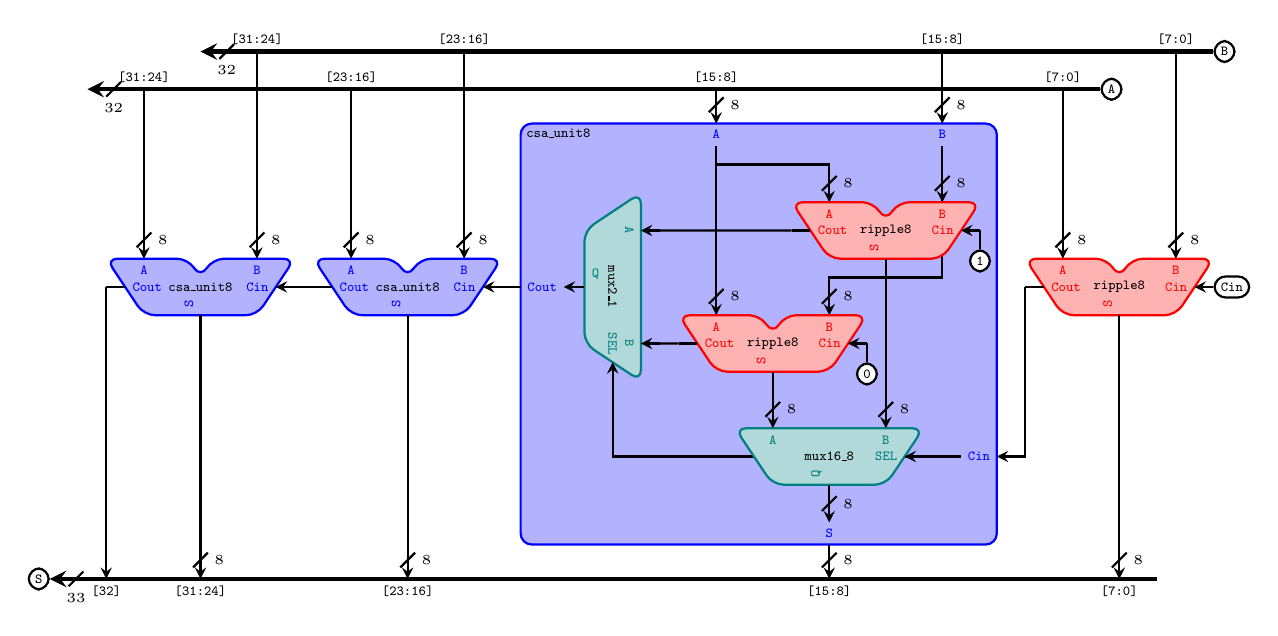
\begin{tikzpicture}[
		>=stealth,
		multiplexer/.pic={
			\coordinate (-O) at (0,0);
			\coordinate (-A) at (-3em,2.5em);
			\coordinate (-B) at (3em,2.5em);
			\coordinate (-SEL) at (5em,0);
			\coordinate (-Q) at (0,-2.5em);
			\draw [pic actions] (-3em,-1.5em) -- (3em,-1.5em) -- (5em,1.5em) -- (-5em,1.5em) --cycle;
			\draw [->,pic actions,fill=black,draw=black] (-A) -- (-3em,1.5em);
			\draw [->,pic actions,fill=black,draw=black] (-B) -- (3em,1.5em);
			\draw [->,pic actions,fill=black,draw=black] (-SEL) -- (4em,0);
			\draw [pic actions,draw=black] (0,-1.5em) -- (-Q);
			\node [anchor=center,text=black] (-center) {\tt\tikzpictext};
			\node [anchor=north] at (-3em,1.5em) {\tiny\tt{A}};
			\node [anchor=north] at (3em,1.5em) {\tiny\tt{B}};
			\node [rotate=90,anchor=south west] at (0,-1.5em) {\tiny\tt{Q}};
			\node [anchor=east] at (4em,0) {\tiny\tt{SEL}};
	  	},
		adder/.pic={
			\coordinate (-O) at (0,0);
			\coordinate (-A) at (-3em,2.5em);
			\coordinate (-B) at (3em,2.5em);
			\coordinate (-Cin) at (5em,0);
			\coordinate (-Cout) at (-5em,0);
			\coordinate (-S) at (0,-2.5em);
			\draw [pic actions] (-3em,-1.5em) -- (3em,-1.5em) -- (5em,1.5em) -- (0.66em,1.5em) -- (0,0.5em) -- (-0.66em,1.5em) -- (-5em,1.5em) --cycle;
			\draw [->,pic actions,fill=black,draw=black] (-A) -- (-3em,1.5em);
			\draw [->,pic actions,fill=black,draw=black] (-B) -- (3em,1.5em);
			\draw [->,pic actions,fill=black,draw=black] (-Cin) -- (4em,0);
			\draw [pic actions,fill=black,draw=black] (-4em,0) -- (-Cout);
			\draw [pic actions,draw=black] (0,-1.5em) -- (-S);
			\node [anchor=center,text=black] (-center) {\tt\tikzpictext};
			\node [anchor=north] at (-3em,1.5em) {\tiny\tt{A}};
			\node [anchor=north] at (3em,1.5em) {\tiny\tt{B}};
			\node [rotate=90,anchor=south west] at (0,-1.5em) {\tiny\tt{S}};
			\node [anchor=east] at (4em,0) {\tiny\tt{Cin}};
			\node [anchor=west] at (-4em,0) {\tiny\tt{Cout}};
	  	}
	]\tiny
		\pic ["mux16\_8",thick,draw=teal,fill=teal!30,text=teal,rounded corners] (smux) {multiplexer};

		\node [draw,strike out,thick,minimum size=0.1] (bus-S0) at (smux-A) {};
		\node [draw,strike out,thick,minimum size=0.1] (bus-S1) at (smux-B) {};
		\node [draw,strike out,thick,minimum size=0.1] (bus-S) at (smux-Q) {};
		\node [anchor=west] at (bus-S0.east) {8};
		\node [anchor=west] at (bus-S1.east) {8};
		\node [anchor=west] at (bus-S.east) {8};

		\pic ["ripple8",thick,draw=red,fill=red!30,text=red,rounded corners,above=3.5em of smux-A] (ra0) {adder};

		\node [draw,strike out,thick,minimum size=0.1] (bus-A) at (ra0-A) {};
		\node [draw,strike out,thick,minimum size=0.1] (bus-B) at (ra0-B) {};
		\node [anchor=west] at (bus-A.east) {8};
		\node [anchor=west] at (bus-B.east) {8};

		\pic ["ripple8",thick,draw=red,fill=red!30,text=red,rounded corners,above=9.5em of smux-B] (ra1) {adder};

		\node [draw,strike out,thick,minimum size=0.1] (bus-A) at (ra1-A) {};
		\node [draw,strike out,thick,minimum size=0.1] (bus-B) at (ra1-B) {};
		\node [anchor=west] at (bus-A.east) {8};
		\node [anchor=west] at (bus-B.east) {8};

		\pic ["mux2\_1",thick,draw=teal,fill=teal!30,text=teal,rounded corners,rotate=-90,transform shape,left=6.5em of $(ra0-Cout)!0.5!(ra1-Cout)$] (cmux) {multiplexer};

		\node [draw,fill=white,thick,rectangle,rounded corners,below=1em of ra0-Cin] (0) {\tt{0}};
		\node [draw,fill=white,thick,rectangle,rounded corners,below=1em of ra1-Cin] (1) {\tt{1}};

		\node [text=blue,above=8em of ra0-A] (unit1-A) {\tt{A}};
		\node [text=blue,above=2em of ra1-B] (unit1-B) {\tt{B}};
		\node [text=blue,right=2em of smux-SEL] (unit1-Cin) {\tt{Cin}};

		\node [text=blue,left=0.1em of cmux-Q] (unit1-Cout) {\tt{Cout}};
		\node [text=blue,below=1em of smux-Q] (unit1-S) {\tt{S}};

		\begin{pgfonlayer}{background}
			\node [draw=blue,fill=blue!30,thick,rectangle,rounded corners,inner sep=0,fit=(unit1-A) (unit1-B) (unit1-Cin) (unit1-Cout) (unit1-S)] (unit1) {};

			\node [anchor=north west,rounded corners,rectangle] at (unit1.north west) {\tt{csa\_unit8}};

			\draw [thick] (ra0-Cin) -- (0);
			\draw [thick] (ra1-Cin) -- (1);

			\draw [thick] (ra0-A) -- (unit1-A);
			\draw [thick] (ra1-A) -- ($(ra1-A) + (0,1em)$) -| (unit1-A);

			\draw [thick] (ra0-B) -- ($(ra0-B) + (0,1em)$) -| (unit1-B);
			\draw [thick] (ra1-B) -- (unit1-B);

			\draw [thick] (ra0-S) -- (smux-A);
			\draw [thick] (ra1-S) -- (smux-B);

			\draw [thick] (ra0-Cout) -- (cmux-B);
			\draw [thick] (ra1-Cout) -- (cmux-A);

			\draw [thick] (cmux-SEL) |- (unit1-Cin);
			\draw [thick] (smux-SEL) -- (unit1-Cin);

			\draw [->,thick] (cmux-Q) -- (unit1-Cout);
			\draw [->,thick] (smux-Q) -- (unit1-S);
		\end{pgfonlayer}

		\pic ["ripple8",thick,draw=red,fill=red!30,text=red,rounded corners,right=29.5em of unit1-Cout] (unit0) {adder};

		\pic ["csa\_unit8",thick,draw=blue,fill=blue!30,text=blue,rounded corners,left=6em of unit1-Cout] (unit2) {adder};
		\pic ["csa\_unit8",thick,draw=blue,fill=blue!30,text=blue,rounded corners,left=6em of unit2-Cout] (unit3) {adder};

		\node [above=8em of unit3-A] (A3) {\tiny\tt{[31:24]}};
		\node [above=8em of unit2-A] (A2) {\tiny\tt{[23:16]}};
		\node [above=3em of unit1-A.south] (A1) {\tiny\tt{[15:8]}};
		\node [above=8em of unit0-A] (A0) {\tiny\tt{[7:0]}};
		\node [left=3em of A3.south] (A-end) {};
		\node [draw,thick,rectangle,rounded corners,right=2em of A0.south] (A-start) {\tt{A}};

		\node [above=10em of unit3-B] (B3) {\tiny\tt{[31:24]}};
		\node [above=10em of unit2-B] (B2) {\tiny\tt{[23:16]}};
		\node [above=5em of unit1-B.south] (B1) {\tiny\tt{[15:8]}};
		\node [above=10em of unit0-B] (B0) {\tiny\tt{[7:0]}};
		\node [left=3em of B3.south] (B-end) {};
		\node [draw,thick,rectangle,rounded corners,right=2em of B0.south] (B-start) {\tt{B}};

		\node [below=15.5em of unit3-Cout] (S4) {\tiny\tt{[32]}};
		\node [below=13em of unit3-S] (S3) {\tiny\tt{[31:24]}};
		\node [below=13em of unit2-S] (S2) {\tiny\tt{[23:16]}};
		\node [below=3em of unit1-S.north] (S1) {\tiny\tt{[15:8]}};
		\node [below=13em of unit0-S] (S0) {\tiny\tt{[7:0]}};
		\node [draw,thick,rectangle,rounded corners,left=3em of S4.north] (S-end) {\tt{S}};
		\node [right=2em of S0.north] (S-start) {};

		\node [draw,thick,rectangle,rounded corners,anchor=west] at (unit0-Cin) {\tt{Cin}};

		\node [draw,strike out,thick,minimum size=0.1] at (unit0-A) (bus-A) {};
		\node [draw,strike out,thick,minimum size=0.1] at (unit0-B) (bus-B) {};
		\node [draw,strike out,thick,minimum size=0.1,above=1em of S0,anchor=center] (bus-S) {};
		\node [anchor=west] at (bus-A.east) {8};
		\node [anchor=west] at (bus-B.east) {8};
		\node [anchor=west] at (bus-S.east) {8};

		\node [draw,strike out,thick,minimum size=0.1,above=1em of unit1-A,anchor=center] (bus-A) {};
		\node [draw,strike out,thick,minimum size=0.1,above=1em of unit1-B,anchor=center] (bus-B) {};
		\node [draw,strike out,thick,minimum size=0.1,above=1em of S1,anchor=center] (bus-S) {};
		\node [anchor=west] at (bus-A.east) {8};
		\node [anchor=west] at (bus-B.east) {8};
		\node [anchor=west] at (bus-S.east) {8};

		\node [draw,strike out,thick,minimum size=0.1] at (unit2-A) (bus-A) {};
		\node [draw,strike out,thick,minimum size=0.1] at (unit2-B) (bus-B) {};
		\node [draw,strike out,thick,minimum size=0.1,above=1em of S2,anchor=center] (bus-S) {};
		\node [anchor=west] at (bus-A.east) {8};
		\node [anchor=west] at (bus-B.east) {8};
		\node [anchor=west] at (bus-S.east) {8};

		\node [draw,strike out,thick,minimum size=0.1] at (unit3-A) (bus-A) {};
		\node [draw,strike out,thick,minimum size=0.1] at (unit3-B) (bus-B) {};
		\node [draw,strike out,thick,minimum size=0.1,above=1em of S3,anchor=center] (bus-S) {};
		\node [anchor=west] at (bus-A.east) {8};
		\node [anchor=west] at (bus-B.east) {8};
		\node [anchor=west] at (bus-S.east) {8};

		\node [draw,strike out,thick,minimum size=0.1,right=1em of A-end] (bus-A) {};
		\node [draw,strike out,thick,minimum size=0.1,right=1em of B-end] (bus-B) {};
		\node [draw,strike out,thick,minimum size=0.1,right=1em of S-end] (bus-S) {};
		\node [anchor=north] at (bus-A.south) {32};
		\node [anchor=north] at (bus-B.south) {32};
		\node [anchor=north] at (bus-S.south) {33};

		\begin{pgfonlayer}{background}
			\draw [->,ultra thick] (A-start) -- (A-end);
			\draw [->,ultra thick] (B-start) -- (B-end);
			\draw [->,ultra thick] (S-start) -- (S-end);

			\draw [->,thick] (unit0-Cout) |- (unit1-Cin);
			\draw [thick] (unit1-Cout) -- (unit2-Cin);
			\draw [thick] (unit2-Cout) -- (unit3-Cout);

			\draw [thick] (A0) -- (unit0-A);
			\draw [->,thick] (A1) -- (unit1-A);
			\draw [thick] (A2) -- (unit2-A);
			\draw [thick] (A3) -- (unit3-A);

			\draw [thick] (B0) -- (unit0-B);
			\draw [->,thick] (B1) -- (unit1-B);
			\draw [thick] (B2) -- (unit2-B);
			\draw [thick] (B3) -- (unit3-B);

			\draw [->,thick] (unit0-S) -- (S0);
			\draw [->,thick] (unit1-S) -- (S1);
			\draw [->,thick] (unit2-S) -- (S2);
			\draw [->,thick] (unit3-S) -- (S3);
			\draw [->,thick] (unit3-Cout) -- (S4);
		\end{pgfonlayer}
	\end{tikzpicture}
	\hspace{-\textwidth}
	\caption{Diagram of a 32-bit carry select adder, with 8-bit select units}
	\label{fig:csa}
\end{figure}

Figure~\ref{fig:hierarchy} illustrates the hierarchy of files used to build the 32-bit CSA in Figure~\ref{fig:csa} and a 32-bit CRA which was used as a reference. Both The CSA and CRA were implemented in \Altera \QuartusII and shared as much VHDL as possible to avoid discrepencies in implementation efficiency. Only the top-level files used the \QuartusII block schematic file format.

\begin{figure}[!h]
	\centering
	\footnotesize
	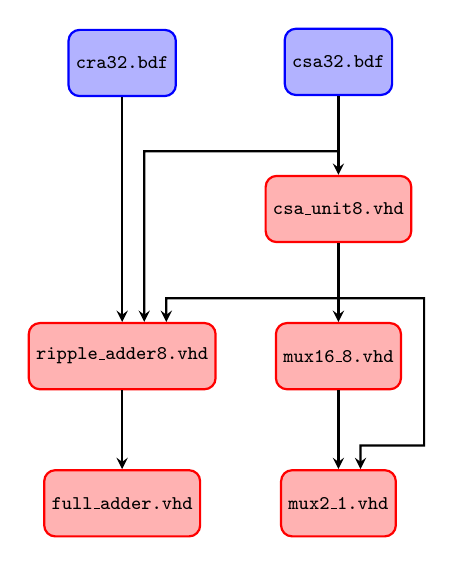
\begin{tikzpicture}[
		>=stealth,
		vhdl/.style={draw=red,fill=red!30,thick,rectangle,rounded corners,minimum size=3em},
		block/.style={draw=blue,fill=blue!30,thick,rectangle,rounded corners,minimum size=3em},
		inv/.style={draw=none,fill=none,rectangle,minimum size=3em}
	]\scriptsize
		\node [vhdl] (full_adder) {\texttt{full\_adder.vhd}};
		\node [vhdl,above=of full_adder] (ripple_adder8) {\texttt{ripple\_adder8.vhd}};
		\node [inv,above=of ripple_adder8] (inv) {};
		\node [block,above=of inv] (cra32) {\texttt{cra32.bdf}};

		\node [vhdl,right=of full_adder] (mux2_1) {\texttt{mux2\_1.vhd}};
		\node [vhdl,above=of mux2_1] (mux16_8) {\texttt{mux16\_8.vhd}};
		\node [vhdl,above=of mux16_8] (csa_unit8) {\texttt{csa\_unit8.vhd}};
		\node [block,above=of csa_unit8] (csa32) {\texttt{csa32.bdf}};

		\draw [->,thick] (mux16_8) -- (mux2_1);
		\draw [->,thick] (csa_unit8) -- (mux16_8);
		\draw [->,thick] (csa_unit8)
			-- ($(csa_unit8.south)!0.7!(mux16_8.north)$)
			-| ($(ripple_adder8.north) + (2em,0)$);
		\draw [->,thick] (csa_unit8)
			-- ($(csa_unit8.south)!0.7!(mux16_8.north)$)
			-| ($(mux16_8.east) + (1em,0)$)
			|- ($(mux16_8.south)!0.7!(mux2_1.north) + (1em,0)$)
			-- ($(mux2_1.north) + (1em,0)$);
		\draw [->,thick] (csa32) -- (csa_unit8);
		\draw [->,thick] (csa32)
			-- ($(csa32.south)!0.7!(csa_unit8.north)$)
			-| ($(ripple_adder8.north) + (1em,0)$);

		\draw [->,thick] (cra32) -- (ripple_adder8);
		\draw [->,thick] (ripple_adder8) -- (full_adder);
	\end{tikzpicture}
	\caption{Hierarchy of entity declarations}
	\label{fig:hierarchy}
\end{figure}

Listings~\ref{lst:full_adder}~and~\ref{lst:mux2_1} include the logic used to implement the \texttt{full\_adder} and \texttt{mux2\_1} entities.

\begin{center}
	\hspace{-\textwidth}%
	\begin{minipage}{0.6\textwidth}
		\lstinputlisting[
			caption={Architecture declaration in \texttt{full\_adder.vhd}},
			label={lst:full_adder},
			language=VHDL,
			style=mystyle,
			firstline=17,
			firstnumber=17,
		]{../quartus/full_adder.vhd}
	\end{minipage}%
	\hspace{2em}%
	\begin{minipage}{0.51\textwidth}
		\lstinputlisting[
			caption={Architecture declaration in \texttt{mux2\_1.vhd}},
			label={lst:mux2_1},
			language=VHDL,
			style=mystyle,
			firstline=15,
			firstnumber=15,
		]{../quartus/mux2_1.vhd}
	\end{minipage}%
	\hspace{-\textwidth}

\end{center}

The 16-to-8 multiplexer was constructed using eight parallel \texttt{mux2\_1} components, mapped to the elements of \texttt{std\_logic\_vector(7 downto 1)} type ports. A similar approach was used to create the 8-bit ripple adder out of \texttt{full\_adder} components. The carry in and carry out were mapped to intermediate \texttt{std\_logic} signals. Signals were also used to represent the candidate sum and carry out values from the 8-bit ripple adders detailed in the \texttt{csa\_unit8} cells in Figure~\ref{fig:csa}.

The top-level entities shown in Figure~\ref{fig:top-level} were built out of \texttt{ripple\_adder8} and \texttt{csa\_unit8} components.

\begin{figure}[!h]
	\centering
	\footnotesize
	\begin{subfigure}[b]{\textwidth}
		\makebox[\textwidth][c]{\includegraphics[width=1.3\textwidth,trim={82pt 680pt 82pt 104pt},clip]{results/cra32.pdf}}%
		\caption{\texttt{cra32.bdf}: 32-bit carry ripple adder}
		\label{fig:cra32.bdf}
	\end{subfigure}
	\begin{subfigure}[b]{\textwidth}
		\makebox[\textwidth][c]{\includegraphics[width=1.3\textwidth,trim={82pt 678pt 82pt 104pt},clip]{results/csa32.pdf}}%
		\caption{\texttt{csa32.bdf}: 32-bit carry select adder, 8-bit select units}
		\label{fig:csa32.bdf}
	\end{subfigure}
	\caption{Block diagram schematics for the top-level entities of each project}
	\label{fig:top-level}
\end{figure}

\section{Speed and Operation}

The verify the correct operation of the CSA circuit under investigation and the CRA reference circuit, a functional simulation was run on the each project. The circuits were compiled for an FPGA: the \Altera Cyclone EP1C20F400C7.

Figure~\ref{fig:func-sim} displays the results of the simulation, with the inputs designed to achieve \SI{100}{\percent} coverage of 0/1 and 1/0 transitions for all nodes. The circuit outputs and coverage statistics were verified in the simulation report.

\begin{figure}[!h]
	\begin{tikztimingtable}[
		timing/xunit=3.2em,
		timing/yunit=0.6em,
	    timing/lslope=0.05,
	    timing/dslope=0.05,
	    timing/font=\ttfamily\footnotesize,
	    timing/text format=\ttfamily\footnotesize,
	    timing/initchar=Z,
	    timing/d/.style={fill=white},
	    timing/z/.style={draw=none},
	    thick
	]
		A[31:0] & 0Z
			D{0000\,0000}
			D{0000\,0001}
			D{FFFF\,FFFF}
			D{0000\,0000}
			D{0101\,0101}
	 		D{7F7F\,7F7F}
			D{0000\,0000}
			D{FFFF\,FFFF}
			2D{0000\,0000}
			D{FFFF\,FFFF}
			0Z \\
		B[31:0] & 0Z
			D{0000\,0000}
			D{FFFF\,FFFF}
			D{0000\,0001}
			D{0000\,0000}
			D{7F7F\,7F7F}
	 		D{0101\,0101}
			2D{0000\,0000}
			D{FFFF\,FFFF}
			D{0000\,0000}
			D{FFFF\,FFFF}
			0Z \\
		CIN~~~~ &
			7L
			2H
			L
			H
			\\
		cra32.qpf:\,S[32:0] & 0Z
			D{0\,0000\,0000}
			2D{1\,0000\,0000}
			D{0\,0000\,0000}
			2D{0\,8080\,8080}
			D{0\,0000\,0000}
			2D{1\,0000\,0000}
			D{0\,0000\,0000}
			D{1\,FFFF\,FFFF}
			0Z \\
		csa32.qpf:\,S[32:0] & 0Z
			D{0\,0000\,0000}
			2D{1\,0000\,0000}
			D{0\,0000\,0000}
			2D{0\,8080\,8080}
			D{0\,0000\,0000}
			2D{1\,0000\,0000}
			D{0\,0000\,0000}
			D{1\,FFFF\,FFFF}
			0Z \\
	\extracode
	\begin{pgfonlayer}{background}
		\fill [lightgray] (0,1.5) rectangle (\twidth,-4.5);
		\draw[decorate,decoration={brace,raise=0.6em}]
			(0,-4.5) -- node[left=1.6em,rotate=90,anchor=center] {\tt{test.vwf}} (0,1.5);
		\vertlines[darkgray,dotted]{0,1,...,\twidth};
	\end{pgfonlayer}
	\end{tikztimingtable}
	\caption{Functional simulation output, \SI{100}{\percent} coverage}
	\label{fig:func-sim}
\end{figure}

The same test vector was used to compare the speed of the CRA and CSA circuits. A timing simulation was run and the transitions with the longest propagation delay were compared. The results of these simulations can be seen in Figure~\ref{fig:time-sim}.

\begin{figure}[!h]
	\centering
	\footnotesize
	\setlength{\pgfsnakesegmentlength}{0.16em}
	\setlength{\pgfsnakesegmentamplitude}{0.15em}
	\begin{subfigure}[t]{0.5\textwidth}
		\centering
		\begin{tikztimingtable}[
			timing/xunit=3.2em/20,
			timing/yunit=0.6em,
		    timing/lslope=0.05*20,
		    timing/dslope=0.05*20,
		    timing/font=\ttfamily\footnotesize,
		    timing/text format=\ttfamily\footnotesize,
		    timing/initchar=Z,
		    timing/d/.style={fill=white},
		    timing/z/.style={draw=none},
		    timing/m/.style={draw=black,snake=zigzag},
		    thick
		]
			A[31:0] &
				25D{0000\,0000}
				100D{0000\,0001}
				0Z \\
			B[31:0] &
				25D{0000\,0000}
				100D{FFFF\,FFFF}
				0Z \\
			CIN &
				125L
				\\
			S[32:0] &
				34.119D{0\,0000\,0000}
				49.006M
				41.875D{1\,0000\,0000}
				0Z \\
			S[32] &
				25L 	9.119L 	0.117L 	0.034L 	0.175L 	0.133L 	0.211L 	0.004L 	0.069L 	0.223L 	0.433L 	0.496L 	0.43L 	0.133L 	0.126L 	0.115L 	0.098L 	0.092L 	0.017L 	0.192L 	0.028L 	0.023L 	0.044L 	0.008L 	0.182L 	0.026L 	0.009L 	0.034L 	0.067L 	0.196L 	0.338L 	0.065L 	0.118L 	0.403L 	0.091L 	0.294L 	0.15L 	1.211L 	5.206L 	0.704L 	0.651L 	1.007L 	1.119L 	4.608L 	3.812L 	0.059L 	1.536L 	0.198L 	1.189L 	2.995L 	0.365L 	3.575L 	0.295L 	0.628L 	2.329L 	1.237L 	0.5L 	0.631L 	0.297L 	1.302L 	5.107L 	0.332L 	0.346L 	0.556L 	0.268L 	1.769H 	41.875H 
				\\
			S[31] &
				25L 	9.119L 	0.117L 	0.034L 	0.175L 	0.133L 	0.211L 	0.004L 	0.069L 	0.223L 	0.433L 	0.496L 	0.43L 	0.133L 	0.126H 	0.115H 	0.098H 	0.092H 	0.017H 	0.192H 	0.028H 	0.023H 	0.044H 	0.008H 	0.182H 	0.026H 	0.009H 	0.034H 	0.067H 	0.196H 	0.338H 	0.065H 	0.118H 	0.403H 	0.091H 	0.294H 	0.15H 	1.211H 	5.206H 	0.704H 	0.651H 	1.007H 	1.119H 	4.608H 	3.812H 	0.059H 	1.536H 	0.198H 	1.189H 	2.995H 	0.365H 	3.575H 	0.295H 	0.628H 	2.329H 	1.237H 	0.5H 	0.631H 	0.297H 	1.302H 	5.107H 	0.332H 	0.346H 	0.556H 	0.268L 	1.769L 	41.875L 
				\\
			S[30] &
				25L 	9.119L 	0.117L 	0.034L 	0.175L 	0.133L 	0.211L 	0.004L 	0.069L 	0.223L 	0.433L 	0.496L 	0.43L 	0.133L 	0.126L 	0.115L 	0.098L 	0.092L 	0.017L 	0.192L 	0.028L 	0.023L 	0.044L 	0.008L 	0.182L 	0.026L 	0.009L 	0.034L 	0.067L 	0.196L 	0.338L 	0.065L 	0.118L 	0.403L 	0.091L 	0.294H 	0.15H 	1.211H 	5.206H 	0.704H 	0.651H 	1.007H 	1.119H 	4.608H 	3.812H 	0.059H 	1.536H 	0.198H 	1.189H 	2.995H 	0.365H 	3.575H 	0.295H 	0.628H 	2.329H 	1.237H 	0.5H 	0.631H 	0.297H 	1.302H 	5.107H 	0.332H 	0.346H 	0.556H 	0.268H 	1.769H 	41.875L 
				\\
			S[29] &
				25L 	9.119L 	0.117L 	0.034L 	0.175L 	0.133L 	0.211L 	0.004L 	0.069L 	0.223L 	0.433L 	0.496L 	0.43L 	0.133L 	0.126L 	0.115L 	0.098L 	0.092L 	0.017L 	0.192L 	0.028L 	0.023L 	0.044L 	0.008L 	0.182L 	0.026L 	0.009L 	0.034H 	0.067H 	0.196H 	0.338H 	0.065H 	0.118H 	0.403H 	0.091H 	0.294H 	0.15H 	1.211H 	5.206H 	0.704H 	0.651H 	1.007H 	1.119H 	4.608H 	3.812H 	0.059H 	1.536H 	0.198H 	1.189H 	2.995H 	0.365H 	3.575H 	0.295H 	0.628H 	2.329H 	1.237H 	0.5H 	0.631H 	0.297H 	1.302H 	5.107H 	0.332H 	0.346L 	0.556L 	0.268L 	1.769L 	41.875L 
				\\
			S[28] &
				25L 	9.119L 	0.117L 	0.034L 	0.175L 	0.133L 	0.211L 	0.004L 	0.069L 	0.223L 	0.433L 	0.496L 	0.43L 	0.133L 	0.126L 	0.115L 	0.098L 	0.092L 	0.017L 	0.192L 	0.028L 	0.023L 	0.044H 	0.008H 	0.182H 	0.026H 	0.009H 	0.034H 	0.067H 	0.196H 	0.338H 	0.065H 	0.118H 	0.403H 	0.091H 	0.294H 	0.15H 	1.211H 	5.206H 	0.704H 	0.651H 	1.007H 	1.119H 	4.608H 	3.812H 	0.059H 	1.536H 	0.198H 	1.189H 	2.995H 	0.365H 	3.575H 	0.295H 	0.628H 	2.329H 	1.237H 	0.5H 	0.631H 	0.297H 	1.302H 	5.107H 	0.332H 	0.346H 	0.556L 	0.268L 	1.769L 	41.875L 
				\\
			S[27] &
				25L 	9.119L 	0.117L 	0.034L 	0.175L 	0.133L 	0.211L 	0.004L 	0.069L 	0.223L 	0.433L 	0.496L 	0.43L 	0.133L 	0.126L 	0.115L 	0.098L 	0.092L 	0.017L 	0.192L 	0.028L 	0.023L 	0.044L 	0.008L 	0.182L 	0.026L 	0.009L 	0.034L 	0.067L 	0.196L 	0.338L 	0.065L 	0.118H 	0.403H 	0.091H 	0.294H 	0.15H 	1.211H 	5.206H 	0.704H 	0.651H 	1.007H 	1.119H 	4.608H 	3.812H 	0.059H 	1.536H 	0.198H 	1.189H 	2.995H 	0.365H 	3.575H 	0.295H 	0.628H 	2.329H 	1.237H 	0.5H 	0.631H 	0.297H 	1.302H 	5.107H 	0.332L 	0.346L 	0.556L 	0.268L 	1.769L 	41.875L 
				\\
			S[26] &
				25L 	9.119L 	0.117L 	0.034L 	0.175L 	0.133L 	0.211L 	0.004L 	0.069L 	0.223L 	0.433L 	0.496L 	0.43L 	0.133L 	0.126L 	0.115L 	0.098L 	0.092L 	0.017L 	0.192L 	0.028L 	0.023L 	0.044L 	0.008H 	0.182H 	0.026H 	0.009H 	0.034H 	0.067H 	0.196H 	0.338H 	0.065H 	0.118H 	0.403H 	0.091H 	0.294H 	0.15H 	1.211H 	5.206H 	0.704H 	0.651H 	1.007H 	1.119H 	4.608H 	3.812H 	0.059H 	1.536H 	0.198H 	1.189H 	2.995H 	0.365H 	3.575H 	0.295H 	0.628H 	2.329H 	1.237H 	0.5H 	0.631H 	0.297H 	1.302H 	5.107L 	0.332L 	0.346L 	0.556L 	0.268L 	1.769L 	41.875L 
				\\
			S[25] &
				25L 	9.119L 	0.117L 	0.034L 	0.175L 	0.133L 	0.211L 	0.004L 	0.069L 	0.223L 	0.433L 	0.496L 	0.43H 	0.133H 	0.126H 	0.115H 	0.098H 	0.092H 	0.017H 	0.192H 	0.028H 	0.023H 	0.044H 	0.008H 	0.182H 	0.026H 	0.009H 	0.034H 	0.067H 	0.196H 	0.338H 	0.065H 	0.118H 	0.403H 	0.091H 	0.294H 	0.15H 	1.211H 	5.206H 	0.704H 	0.651H 	1.007H 	1.119H 	4.608H 	3.812H 	0.059H 	1.536H 	0.198H 	1.189H 	2.995H 	0.365H 	3.575H 	0.295H 	0.628H 	2.329H 	1.237H 	0.5H 	0.631H 	0.297L 	1.302L 	5.107L 	0.332L 	0.346L 	0.556L 	0.268L 	1.769L 	41.875L 
				\\
			S[24] &
				25L 	9.119L 	0.117L 	0.034L 	0.175L 	0.133H 	0.211H 	0.004H 	0.069H 	0.223H 	0.433H 	0.496H 	0.43H 	0.133H 	0.126H 	0.115H 	0.098H 	0.092H 	0.017H 	0.192H 	0.028H 	0.023H 	0.044H 	0.008H 	0.182H 	0.026H 	0.009H 	0.034H 	0.067H 	0.196H 	0.338H 	0.065H 	0.118H 	0.403H 	0.091H 	0.294H 	0.15H 	1.211H 	5.206H 	0.704H 	0.651H 	1.007H 	1.119H 	4.608H 	3.812H 	0.059H 	1.536H 	0.198H 	1.189H 	2.995H 	0.365H 	3.575H 	0.295H 	0.628H 	2.329H 	1.237H 	0.5H 	0.631H 	0.297H 	1.302L 	5.107L 	0.332L 	0.346L 	0.556L 	0.268L 	1.769L 	41.875L 
				\\
			S[23] &
				25L 	9.119L 	0.117L 	0.034L 	0.175L 	0.133L 	0.211L 	0.004L 	0.069L 	0.223L 	0.433L 	0.496L 	0.43L 	0.133L 	0.126L 	0.115L 	0.098L 	0.092H 	0.017H 	0.192H 	0.028H 	0.023H 	0.044H 	0.008H 	0.182H 	0.026H 	0.009H 	0.034H 	0.067H 	0.196H 	0.338H 	0.065H 	0.118H 	0.403H 	0.091H 	0.294H 	0.15H 	1.211H 	5.206H 	0.704H 	0.651H 	1.007H 	1.119H 	4.608H 	3.812H 	0.059H 	1.536H 	0.198H 	1.189H 	2.995H 	0.365H 	3.575H 	0.295H 	0.628H 	2.329H 	1.237H 	0.5H 	0.631L 	0.297L 	1.302L 	5.107L 	0.332L 	0.346L 	0.556L 	0.268L 	1.769L 	41.875L 
				\\
			S[22] &
				25L 	9.119L 	0.117H 	0.034H 	0.175H 	0.133H 	0.211H 	0.004H 	0.069H 	0.223H 	0.433H 	0.496H 	0.43H 	0.133H 	0.126H 	0.115H 	0.098H 	0.092H 	0.017H 	0.192H 	0.028H 	0.023H 	0.044H 	0.008H 	0.182H 	0.026H 	0.009H 	0.034H 	0.067H 	0.196H 	0.338H 	0.065H 	0.118H 	0.403H 	0.091H 	0.294H 	0.15H 	1.211H 	5.206H 	0.704H 	0.651H 	1.007H 	1.119H 	4.608H 	3.812H 	0.059H 	1.536H 	0.198H 	1.189H 	2.995H 	0.365H 	3.575H 	0.295H 	0.628H 	2.329H 	1.237H 	0.5L 	0.631L 	0.297L 	1.302L 	5.107L 	0.332L 	0.346L 	0.556L 	0.268L 	1.769L 	41.875L 
				\\
			S[21] &
				25L 	9.119L 	0.117L 	0.034L 	0.175L 	0.133L 	0.211L 	0.004L 	0.069L 	0.223L 	0.433L 	0.496L 	0.43L 	0.133H 	0.126H 	0.115H 	0.098H 	0.092H 	0.017H 	0.192H 	0.028H 	0.023H 	0.044H 	0.008H 	0.182H 	0.026H 	0.009H 	0.034H 	0.067H 	0.196H 	0.338H 	0.065H 	0.118H 	0.403H 	0.091H 	0.294H 	0.15H 	1.211H 	5.206H 	0.704H 	0.651H 	1.007H 	1.119H 	4.608H 	3.812H 	0.059H 	1.536H 	0.198H 	1.189H 	2.995H 	0.365H 	3.575H 	0.295H 	0.628H 	2.329H 	1.237L 	0.5L 	0.631L 	0.297L 	1.302L 	5.107L 	0.332L 	0.346L 	0.556L 	0.268L 	1.769L 	41.875L 
				\\
			S[20] &
				25L 	9.119L 	0.117L 	0.034L 	0.175L 	0.133L 	0.211L 	0.004L 	0.069L 	0.223L 	0.433L 	0.496L 	0.43L 	0.133L 	0.126L 	0.115L 	0.098H 	0.092H 	0.017H 	0.192H 	0.028H 	0.023H 	0.044H 	0.008H 	0.182H 	0.026H 	0.009H 	0.034H 	0.067H 	0.196H 	0.338H 	0.065H 	0.118H 	0.403H 	0.091H 	0.294H 	0.15H 	1.211H 	5.206H 	0.704H 	0.651H 	1.007H 	1.119H 	4.608H 	3.812H 	0.059H 	1.536H 	0.198H 	1.189H 	2.995H 	0.365H 	3.575H 	0.295H 	0.628H 	2.329L 	1.237L 	0.5L 	0.631L 	0.297L 	1.302L 	5.107L 	0.332L 	0.346L 	0.556L 	0.268L 	1.769L 	41.875L 
				\\
			S[19] &
				25L 	9.119L 	0.117L 	0.034L 	0.175L 	0.133L 	0.211L 	0.004L 	0.069L 	0.223L 	0.433L 	0.496L 	0.43L 	0.133L 	0.126L 	0.115L 	0.098L 	0.092L 	0.017L 	0.192L 	0.028L 	0.023L 	0.044L 	0.008L 	0.182L 	0.026L 	0.009L 	0.034L 	0.067L 	0.196L 	0.338H 	0.065H 	0.118H 	0.403H 	0.091H 	0.294H 	0.15H 	1.211H 	5.206H 	0.704H 	0.651H 	1.007H 	1.119H 	4.608H 	3.812H 	0.059H 	1.536H 	0.198H 	1.189H 	2.995H 	0.365H 	3.575H 	0.295H 	0.628L 	2.329L 	1.237L 	0.5L 	0.631L 	0.297L 	1.302L 	5.107L 	0.332L 	0.346L 	0.556L 	0.268L 	1.769L 	41.875L 
				\\
			S[18] &
				25L 	9.119L 	0.117L 	0.034L 	0.175L 	0.133L 	0.211L 	0.004L 	0.069L 	0.223L 	0.433L 	0.496L 	0.43L 	0.133L 	0.126L 	0.115L 	0.098L 	0.092L 	0.017L 	0.192L 	0.028L 	0.023L 	0.044L 	0.008L 	0.182L 	0.026L 	0.009L 	0.034L 	0.067L 	0.196L 	0.338L 	0.065H 	0.118H 	0.403H 	0.091H 	0.294H 	0.15H 	1.211H 	5.206H 	0.704H 	0.651H 	1.007H 	1.119H 	4.608H 	3.812H 	0.059H 	1.536H 	0.198H 	1.189H 	2.995H 	0.365H 	3.575H 	0.295L 	0.628L 	2.329L 	1.237L 	0.5L 	0.631L 	0.297L 	1.302L 	5.107L 	0.332L 	0.346L 	0.556L 	0.268L 	1.769L 	41.875L 
				\\
			S[17] &
				25L 	9.119L 	0.117L 	0.034L 	0.175L 	0.133L 	0.211H 	0.004H 	0.069H 	0.223H 	0.433H 	0.496H 	0.43H 	0.133H 	0.126H 	0.115H 	0.098H 	0.092H 	0.017H 	0.192H 	0.028H 	0.023H 	0.044H 	0.008H 	0.182H 	0.026H 	0.009H 	0.034H 	0.067H 	0.196H 	0.338H 	0.065H 	0.118H 	0.403H 	0.091H 	0.294H 	0.15H 	1.211H 	5.206H 	0.704H 	0.651H 	1.007H 	1.119H 	4.608H 	3.812H 	0.059H 	1.536H 	0.198H 	1.189H 	2.995H 	0.365H 	3.575L 	0.295L 	0.628L 	2.329L 	1.237L 	0.5L 	0.631L 	0.297L 	1.302L 	5.107L 	0.332L 	0.346L 	0.556L 	0.268L 	1.769L 	41.875L 
				\\
			S[16] &
				25L 	9.119L 	0.117L 	0.034L 	0.175L 	0.133L 	0.211L 	0.004L 	0.069L 	0.223L 	0.433L 	0.496L 	0.43L 	0.133L 	0.126L 	0.115L 	0.098L 	0.092L 	0.017L 	0.192L 	0.028H 	0.023H 	0.044H 	0.008H 	0.182H 	0.026H 	0.009H 	0.034H 	0.067H 	0.196H 	0.338H 	0.065H 	0.118H 	0.403H 	0.091H 	0.294H 	0.15H 	1.211H 	5.206H 	0.704H 	0.651H 	1.007H 	1.119H 	4.608H 	3.812H 	0.059H 	1.536H 	0.198H 	1.189H 	2.995H 	0.365L 	3.575L 	0.295L 	0.628L 	2.329L 	1.237L 	0.5L 	0.631L 	0.297L 	1.302L 	5.107L 	0.332L 	0.346L 	0.556L 	0.268L 	1.769L 	41.875L 
				\\
			S[15] &
				25L 	9.119L 	0.117L 	0.034L 	0.175L 	0.133L 	0.211L 	0.004L 	0.069L 	0.223L 	0.433L 	0.496L 	0.43L 	0.133L 	0.126L 	0.115L 	0.098L 	0.092L 	0.017L 	0.192L 	0.028L 	0.023L 	0.044L 	0.008L 	0.182L 	0.026L 	0.009L 	0.034L 	0.067L 	0.196L 	0.338L 	0.065L 	0.118L 	0.403H 	0.091H 	0.294H 	0.15H 	1.211H 	5.206H 	0.704H 	0.651H 	1.007H 	1.119H 	4.608H 	3.812H 	0.059H 	1.536H 	0.198H 	1.189L 	2.995L 	0.365L 	3.575L 	0.295L 	0.628L 	2.329L 	1.237L 	0.5L 	0.631L 	0.297L 	1.302L 	5.107L 	0.332L 	0.346L 	0.556L 	0.268L 	1.769L 	41.875L 
				\\
			S[14] &
				25L 	9.119L 	0.117L 	0.034L 	0.175L 	0.133L 	0.211L 	0.004L 	0.069L 	0.223L 	0.433L 	0.496L 	0.43L 	0.133L 	0.126L 	0.115L 	0.098L 	0.092L 	0.017L 	0.192L 	0.028L 	0.023L 	0.044L 	0.008L 	0.182L 	0.026L 	0.009L 	0.034L 	0.067H 	0.196H 	0.338H 	0.065H 	0.118H 	0.403H 	0.091H 	0.294H 	0.15H 	1.211H 	5.206H 	0.704H 	0.651H 	1.007H 	1.119H 	4.608H 	3.812H 	0.059H 	1.536H 	0.198L 	1.189L 	2.995L 	0.365L 	3.575L 	0.295L 	0.628L 	2.329L 	1.237L 	0.5L 	0.631L 	0.297L 	1.302L 	5.107L 	0.332L 	0.346L 	0.556L 	0.268L 	1.769L 	41.875L 
				\\
			S[13] &
				25L 	9.119L 	0.117L 	0.034L 	0.175L 	0.133L 	0.211L 	0.004L 	0.069L 	0.223L 	0.433L 	0.496L 	0.43L 	0.133L 	0.126L 	0.115L 	0.098L 	0.092L 	0.017L 	0.192H 	0.028H 	0.023H 	0.044H 	0.008H 	0.182H 	0.026H 	0.009H 	0.034H 	0.067H 	0.196H 	0.338H 	0.065H 	0.118H 	0.403H 	0.091H 	0.294H 	0.15H 	1.211H 	5.206H 	0.704H 	0.651H 	1.007H 	1.119H 	4.608H 	3.812H 	0.059H 	1.536H 	0.198H 	1.189H 	2.995L 	0.365L 	3.575L 	0.295L 	0.628L 	2.329L 	1.237L 	0.5L 	0.631L 	0.297L 	1.302L 	5.107L 	0.332L 	0.346L 	0.556L 	0.268L 	1.769L 	41.875L 
				\\
			S[12] &
				25L 	9.119L 	0.117L 	0.034L 	0.175L 	0.133L 	0.211L 	0.004L 	0.069H 	0.223H 	0.433H 	0.496H 	0.43H 	0.133H 	0.126H 	0.115H 	0.098H 	0.092H 	0.017H 	0.192H 	0.028H 	0.023H 	0.044H 	0.008H 	0.182H 	0.026H 	0.009H 	0.034H 	0.067H 	0.196H 	0.338H 	0.065H 	0.118H 	0.403H 	0.091H 	0.294H 	0.15H 	1.211H 	5.206H 	0.704H 	0.651H 	1.007H 	1.119H 	4.608H 	3.812H 	0.059L 	1.536L 	0.198L 	1.189L 	2.995L 	0.365L 	3.575L 	0.295L 	0.628L 	2.329L 	1.237L 	0.5L 	0.631L 	0.297L 	1.302L 	5.107L 	0.332L 	0.346L 	0.556L 	0.268L 	1.769L 	41.875L 
				\\
			S[11] &
				25L 	9.119L 	0.117L 	0.034L 	0.175L 	0.133L 	0.211L 	0.004L 	0.069L 	0.223L 	0.433L 	0.496L 	0.43L 	0.133L 	0.126L 	0.115L 	0.098L 	0.092L 	0.017L 	0.192L 	0.028L 	0.023H 	0.044H 	0.008H 	0.182H 	0.026H 	0.009H 	0.034H 	0.067H 	0.196H 	0.338H 	0.065H 	0.118H 	0.403H 	0.091H 	0.294H 	0.15H 	1.211H 	5.206H 	0.704H 	0.651H 	1.007H 	1.119H 	4.608H 	3.812H 	0.059H 	1.536L 	0.198L 	1.189L 	2.995L 	0.365L 	3.575L 	0.295L 	0.628L 	2.329L 	1.237L 	0.5L 	0.631L 	0.297L 	1.302L 	5.107L 	0.332L 	0.346L 	0.556L 	0.268L 	1.769L 	41.875L 
				\\
			S[10] &
				25L 	9.119L 	0.117L 	0.034L 	0.175L 	0.133L 	0.211L 	0.004L 	0.069L 	0.223L 	0.433L 	0.496H 	0.43H 	0.133H 	0.126H 	0.115H 	0.098H 	0.092H 	0.017H 	0.192H 	0.028H 	0.023H 	0.044H 	0.008H 	0.182H 	0.026H 	0.009H 	0.034H 	0.067H 	0.196H 	0.338H 	0.065H 	0.118H 	0.403H 	0.091H 	0.294H 	0.15H 	1.211H 	5.206H 	0.704H 	0.651H 	1.007H 	1.119H 	4.608H 	3.812L 	0.059L 	1.536L 	0.198L 	1.189L 	2.995L 	0.365L 	3.575L 	0.295L 	0.628L 	2.329L 	1.237L 	0.5L 	0.631L 	0.297L 	1.302L 	5.107L 	0.332L 	0.346L 	0.556L 	0.268L 	1.769L 	41.875L 
				\\
			S[9] &
				25L 	9.119L 	0.117L 	0.034L 	0.175L 	0.133L 	0.211L 	0.004L 	0.069L 	0.223L 	0.433H 	0.496H 	0.43H 	0.133H 	0.126H 	0.115H 	0.098H 	0.092H 	0.017H 	0.192H 	0.028H 	0.023H 	0.044H 	0.008H 	0.182H 	0.026H 	0.009H 	0.034H 	0.067H 	0.196H 	0.338H 	0.065H 	0.118H 	0.403H 	0.091H 	0.294H 	0.15H 	1.211H 	5.206H 	0.704H 	0.651H 	1.007H 	1.119L 	4.608L 	3.812L 	0.059L 	1.536L 	0.198L 	1.189L 	2.995L 	0.365L 	3.575L 	0.295L 	0.628L 	2.329L 	1.237L 	0.5L 	0.631L 	0.297L 	1.302L 	5.107L 	0.332L 	0.346L 	0.556L 	0.268L 	1.769L 	41.875L 
				\\
			S[8] &
				25L 	9.119L 	0.117L 	0.034L 	0.175L 	0.133L 	0.211L 	0.004L 	0.069L 	0.223L 	0.433L 	0.496L 	0.43L 	0.133L 	0.126L 	0.115L 	0.098L 	0.092L 	0.017L 	0.192L 	0.028L 	0.023L 	0.044L 	0.008L 	0.182L 	0.026L 	0.009L 	0.034L 	0.067L 	0.196L 	0.338L 	0.065L 	0.118L 	0.403L 	0.091L 	0.294L 	0.15L 	1.211H 	5.206H 	0.704H 	0.651H 	1.007H 	1.119H 	4.608L 	3.812L 	0.059L 	1.536L 	0.198L 	1.189L 	2.995L 	0.365L 	3.575L 	0.295L 	0.628L 	2.329L 	1.237L 	0.5L 	0.631L 	0.297L 	1.302L 	5.107L 	0.332L 	0.346L 	0.556L 	0.268L 	1.769L 	41.875L 
				\\
			S[7] &
				25L 	9.119L 	0.117L 	0.034L 	0.175L 	0.133L 	0.211L 	0.004L 	0.069L 	0.223L 	0.433L 	0.496L 	0.43L 	0.133L 	0.126L 	0.115L 	0.098L 	0.092L 	0.017L 	0.192L 	0.028L 	0.023L 	0.044L 	0.008L 	0.182L 	0.026H 	0.009H 	0.034H 	0.067H 	0.196H 	0.338H 	0.065H 	0.118H 	0.403H 	0.091H 	0.294H 	0.15H 	1.211H 	5.206H 	0.704H 	0.651H 	1.007L 	1.119L 	4.608L 	3.812L 	0.059L 	1.536L 	0.198L 	1.189L 	2.995L 	0.365L 	3.575L 	0.295L 	0.628L 	2.329L 	1.237L 	0.5L 	0.631L 	0.297L 	1.302L 	5.107L 	0.332L 	0.346L 	0.556L 	0.268L 	1.769L 	41.875L 
				\\
			S[6] &
				25L 	9.119L 	0.117L 	0.034L 	0.175L 	0.133L 	0.211L 	0.004L 	0.069L 	0.223L 	0.433L 	0.496L 	0.43L 	0.133L 	0.126L 	0.115L 	0.098L 	0.092L 	0.017L 	0.192L 	0.028L 	0.023L 	0.044L 	0.008L 	0.182L 	0.026L 	0.009L 	0.034L 	0.067L 	0.196H 	0.338H 	0.065H 	0.118H 	0.403H 	0.091H 	0.294H 	0.15H 	1.211H 	5.206H 	0.704H 	0.651L 	1.007L 	1.119L 	4.608L 	3.812L 	0.059L 	1.536L 	0.198L 	1.189L 	2.995L 	0.365L 	3.575L 	0.295L 	0.628L 	2.329L 	1.237L 	0.5L 	0.631L 	0.297L 	1.302L 	5.107L 	0.332L 	0.346L 	0.556L 	0.268L 	1.769L 	41.875L 
				\\
			S[5] &
				25L 	9.119L 	0.117L 	0.034L 	0.175L 	0.133L 	0.211L 	0.004L 	0.069L 	0.223L 	0.433L 	0.496L 	0.43L 	0.133L 	0.126L 	0.115L 	0.098L 	0.092L 	0.017L 	0.192L 	0.028L 	0.023L 	0.044L 	0.008L 	0.182H 	0.026H 	0.009H 	0.034H 	0.067H 	0.196H 	0.338H 	0.065H 	0.118H 	0.403H 	0.091H 	0.294H 	0.15H 	1.211H 	5.206H 	0.704L 	0.651L 	1.007L 	1.119L 	4.608L 	3.812L 	0.059L 	1.536L 	0.198L 	1.189L 	2.995L 	0.365L 	3.575L 	0.295L 	0.628L 	2.329L 	1.237L 	0.5L 	0.631L 	0.297L 	1.302L 	5.107L 	0.332L 	0.346L 	0.556L 	0.268L 	1.769L 	41.875L 
				\\
			S[4] &
				25L 	9.119L 	0.117L 	0.034H 	0.175H 	0.133H 	0.211H 	0.004H 	0.069H 	0.223H 	0.433H 	0.496H 	0.43H 	0.133H 	0.126H 	0.115H 	0.098H 	0.092H 	0.017H 	0.192H 	0.028H 	0.023H 	0.044H 	0.008H 	0.182H 	0.026H 	0.009H 	0.034H 	0.067H 	0.196H 	0.338H 	0.065H 	0.118H 	0.403H 	0.091H 	0.294H 	0.15L 	1.211L 	5.206L 	0.704L 	0.651L 	1.007L 	1.119L 	4.608L 	3.812L 	0.059L 	1.536L 	0.198L 	1.189L 	2.995L 	0.365L 	3.575L 	0.295L 	0.628L 	2.329L 	1.237L 	0.5L 	0.631L 	0.297L 	1.302L 	5.107L 	0.332L 	0.346L 	0.556L 	0.268L 	1.769L 	41.875L 
				\\
			S[3] &
				25L 	9.119L 	0.117L 	0.034L 	0.175L 	0.133L 	0.211L 	0.004H 	0.069H 	0.223H 	0.433H 	0.496H 	0.43H 	0.133H 	0.126H 	0.115H 	0.098H 	0.092H 	0.017H 	0.192H 	0.028H 	0.023H 	0.044H 	0.008H 	0.182H 	0.026H 	0.009H 	0.034H 	0.067H 	0.196H 	0.338H 	0.065H 	0.118H 	0.403H 	0.091L 	0.294L 	0.15L 	1.211L 	5.206L 	0.704L 	0.651L 	1.007L 	1.119L 	4.608L 	3.812L 	0.059L 	1.536L 	0.198L 	1.189L 	2.995L 	0.365L 	3.575L 	0.295L 	0.628L 	2.329L 	1.237L 	0.5L 	0.631L 	0.297L 	1.302L 	5.107L 	0.332L 	0.346L 	0.556L 	0.268L 	1.769L 	41.875L 
				\\
			S[2] &
				25L 	9.119L 	0.117L 	0.034L 	0.175L 	0.133L 	0.211L 	0.004L 	0.069L 	0.223L 	0.433L 	0.496L 	0.43L 	0.133L 	0.126L 	0.115H 	0.098H 	0.092H 	0.017H 	0.192H 	0.028H 	0.023H 	0.044H 	0.008H 	0.182H 	0.026H 	0.009H 	0.034H 	0.067H 	0.196H 	0.338H 	0.065H 	0.118H 	0.403H 	0.091H 	0.294H 	0.15H 	1.211H 	5.206L 	0.704L 	0.651L 	1.007L 	1.119L 	4.608L 	3.812L 	0.059L 	1.536L 	0.198L 	1.189L 	2.995L 	0.365L 	3.575L 	0.295L 	0.628L 	2.329L 	1.237L 	0.5L 	0.631L 	0.297L 	1.302L 	5.107L 	0.332L 	0.346L 	0.556L 	0.268L 	1.769L 	41.875L 
				\\
			S[1] &
				25L 	9.119L 	0.117L 	0.034L 	0.175H 	0.133H 	0.211H 	0.004H 	0.069H 	0.223H 	0.433H 	0.496H 	0.43H 	0.133H 	0.126H 	0.115H 	0.098H 	0.092H 	0.017H 	0.192H 	0.028H 	0.023H 	0.044H 	0.008H 	0.182H 	0.026H 	0.009L 	0.034L 	0.067L 	0.196L 	0.338L 	0.065L 	0.118L 	0.403L 	0.091L 	0.294L 	0.15L 	1.211L 	5.206L 	0.704L 	0.651L 	1.007L 	1.119L 	4.608L 	3.812L 	0.059L 	1.536L 	0.198L 	1.189L 	2.995L 	0.365L 	3.575L 	0.295L 	0.628L 	2.329L 	1.237L 	0.5L 	0.631L 	0.297L 	1.302L 	5.107L 	0.332L 	0.346L 	0.556L 	0.268L 	1.769L 	41.875L 
				\\
			S[0] &
				25L 	9.119L 	0.117L 	0.034L 	0.175L 	0.133L 	0.211L 	0.004L 	0.069L 	0.223H 	0.433H 	0.496H 	0.43H 	0.133H 	0.126H 	0.115H 	0.098H 	0.092H 	0.017L 	0.192L 	0.028L 	0.023L 	0.044L 	0.008L 	0.182L 	0.026L 	0.009L 	0.034L 	0.067L 	0.196L 	0.338L 	0.065L 	0.118L 	0.403L 	0.091L 	0.294L 	0.15L 	1.211L 	5.206L 	0.704L 	0.651L 	1.007L 	1.119L 	4.608L 	3.812L 	0.059L 	1.536L 	0.198L 	1.189L 	2.995L 	0.365L 	3.575L 	0.295L 	0.628L 	2.329L 	1.237L 	0.5L 	0.631L 	0.297L 	1.302L 	5.107L 	0.332L 	0.346L 	0.556L 	0.268L 	1.769L 	41.875L 
				\\
		\extracode
		\begin{pgfonlayer}{background}
			\fill [lightgray] (0,1.5) rectangle (\twidth,-4.5);
			\coordinate (t0) at (25,1);
			\coordinate (t1) at ($(t0) + (22.065,0)$);
			\coordinate (t2) at ($(t0) + (35.593,0)$);
			\coordinate (t3) at ($(t0) + (45.517,0)$);
			\coordinate (t4) at ($(t0) + (58.125,0)$);
			\coordinate (t5) at ($(t0) + (100,0)$);
			\node [darkgray,rotate=90,anchor=south west,inner ysep=0] at (t0) {\tiny\tt0};
			\node [darkgray,rotate=90,anchor=south west,inner ysep=0] at (t1) {\tiny\tt22.065};
			\node [darkgray,rotate=90,anchor=south west,inner ysep=0] at (t2) {\tiny\tt35.593};
			\node [darkgray,rotate=90,anchor=south west,inner ysep=0] at (t3) {\tiny\tt45.517};
			\node [darkgray,rotate=90,anchor=south west,inner ysep=0] at (t4) {\tiny\tt58.125};
			\node [darkgray,rotate=90,anchor=south west,inner ysep=0] at (t5) {\tiny\tt100.00};
			\vertlines[darkgray,dotted]{
				25,
				25 + 22.065,
				25 + 35.593,
				25 + 47.517,
				25 + 58.125,
				25 + 100,
			};
			\coordinate (tm) at ($(t0) + (9.119,0)$,1);
			\node [darkgray,rotate=90,anchor=south west,inner ysep=0] at (tm) {\tiny\tt9.1190};
			\vertlines[lightgray,dotted]{
				25 + 9.119
			}
		\end{pgfonlayer}
		\end{tikztimingtable}
		\caption{32-bit carry ripple adder}
		\label{fig:cra-time}
	\end{subfigure}\hfill%
	\begin{subfigure}[t]{0.5\textwidth}
		\centering
		\begin{tikztimingtable}[
			timing/xunit=3.2em/20,
			timing/yunit=0.6em,
		    timing/lslope=0.05*20,
		    timing/dslope=0.05*20,
		    timing/font=\ttfamily\footnotesize,
		    timing/text format=\ttfamily\footnotesize,
		    timing/initchar=Z,
		    timing/d/.style={fill=white},
		    timing/z/.style={draw=none},
		    timing/m/.style={draw=black,snake=zigzag},
		    thick
		]
			A[31:0] &
				25D{0000\,0000}
				100D{0000\,0001}
				0Z \\
			B[31:0] &
				25D{0000\,0000}
				100D{FFFF\,FFFF}
				0Z \\
			CIN &
				125L
				 \\
			S[32:0] &
				33.675D{0\,0000\,0000}
				18.913M
				72.412D{1\,0000\,0000}
				0Z \\
			S[32] &
				25L 	8.675L 	0.081L 	0.265L 	0.087L 	0.047L 	0.249L 	0.112L 	0.018L 	0.033L 	0.014L 	0.013L 	0.013L 	0.198L 	0.056L 	0.108L 	0.203L 	0.421L 	0.217L 	0.144L 	0.202L 	0.024L 	0.429L 	0.004L 	0.257L 	0.326L 	0.082L 	0.073L 	0.006L 	0.036L 	0.145L 	0.261L 	0.16L 	0.383L 	0.125L 	0.206L 	0.077L 	0.34L 	0.674L 	0.238L 	1.482L 	0.639L 	0.106L 	0.152L 	0.971L 	0.912L 	0.246L 	0.645L 	1.095L 	0.305L 	0.052L 	0.756L 	0.108L 	0.33L 	0.662L 	0.023L 	0.009L 	0.644L 	0.106L 	0.497H 	0.037H 	0.1H 	1.338H 	1.321H 	0.008H 	0.042H 	72.412H 
				\\
			S[31] &
				25L 	8.675L 	0.081L 	0.265L 	0.087L 	0.047L 	0.249L 	0.112L 	0.018L 	0.033L 	0.014L 	0.013L 	0.013L 	0.198L 	0.056L 	0.108L 	0.203L 	0.421L 	0.217L 	0.144L 	0.202L 	0.024L 	0.429L 	0.004L 	0.257L 	0.326L 	0.082L 	0.073L 	0.006L 	0.036L 	0.145L 	0.261L 	0.16L 	0.383L 	0.125H 	0.206H 	0.077H 	0.34H 	0.674H 	0.238H 	1.482H 	0.639H 	0.106H 	0.152H 	0.971H 	0.912H 	0.246H 	0.645H 	1.095H 	0.305H 	0.052H 	0.756H 	0.108H 	0.33H 	0.662H 	0.023H 	0.009H 	0.644H 	0.106H 	0.497H 	0.037H 	0.1H 	1.338H 	1.321L 	0.008L 	0.042L 	72.412L 
				\\
			S[30] &
				25L 	8.675L 	0.081L 	0.265L 	0.087L 	0.047L 	0.249L 	0.112L 	0.018L 	0.033L 	0.014L 	0.013L 	0.013L 	0.198L 	0.056L 	0.108L 	0.203L 	0.421L 	0.217L 	0.144L 	0.202L 	0.024L 	0.429L 	0.004L 	0.257L 	0.326L 	0.082L 	0.073L 	0.006L 	0.036L 	0.145L 	0.261L 	0.16L 	0.383L 	0.125L 	0.206H 	0.077H 	0.34H 	0.674H 	0.238H 	1.482H 	0.639H 	0.106H 	0.152H 	0.971H 	0.912H 	0.246H 	0.645H 	1.095H 	0.305H 	0.052H 	0.756H 	0.108H 	0.33H 	0.662H 	0.023H 	0.009H 	0.644H 	0.106H 	0.497H 	0.037H 	0.1H 	1.338H 	1.321H 	0.008L 	0.042L 	72.412L 
				\\
			S[29] &
				25L 	8.675L 	0.081L 	0.265L 	0.087L 	0.047L 	0.249L 	0.112L 	0.018H 	0.033H 	0.014H 	0.013H 	0.013H 	0.198H 	0.056H 	0.108H 	0.203H 	0.421H 	0.217H 	0.144H 	0.202H 	0.024H 	0.429H 	0.004H 	0.257H 	0.326H 	0.082H 	0.073H 	0.006H 	0.036H 	0.145H 	0.261H 	0.16H 	0.383H 	0.125H 	0.206H 	0.077H 	0.34H 	0.674H 	0.238H 	1.482H 	0.639H 	0.106H 	0.152H 	0.971H 	0.912H 	0.246H 	0.645H 	1.095H 	0.305H 	0.052H 	0.756H 	0.108H 	0.33H 	0.662H 	0.023H 	0.009H 	0.644H 	0.106H 	0.497H 	0.037L 	0.1L 	1.338L 	1.321L 	0.008L 	0.042L 	72.412L 
				\\
			S[28] &
				25L 	8.675L 	0.081L 	0.265L 	0.087L 	0.047L 	0.249L 	0.112L 	0.018L 	0.033L 	0.014L 	0.013L 	0.013L 	0.198L 	0.056L 	0.108L 	0.203L 	0.421L 	0.217L 	0.144L 	0.202L 	0.024L 	0.429L 	0.004L 	0.257L 	0.326L 	0.082L 	0.073L 	0.006L 	0.036L 	0.145L 	0.261L 	0.16L 	0.383L 	0.125L 	0.206L 	0.077L 	0.34L 	0.674L 	0.238L 	1.482H 	0.639H 	0.106H 	0.152H 	0.971H 	0.912H 	0.246H 	0.645H 	1.095H 	0.305H 	0.052H 	0.756H 	0.108H 	0.33H 	0.662H 	0.023H 	0.009H 	0.644H 	0.106H 	0.497H 	0.037H 	0.1H 	1.338H 	1.321H 	0.008H 	0.042L 	72.412L 
				\\
			S[27] &
				25L 	8.675L 	0.081L 	0.265L 	0.087L 	0.047L 	0.249L 	0.112L 	0.018L 	0.033L 	0.014L 	0.013L 	0.013L 	0.198L 	0.056L 	0.108L 	0.203H 	0.421H 	0.217H 	0.144H 	0.202H 	0.024H 	0.429H 	0.004H 	0.257H 	0.326H 	0.082H 	0.073H 	0.006H 	0.036H 	0.145H 	0.261H 	0.16H 	0.383H 	0.125H 	0.206H 	0.077H 	0.34H 	0.674H 	0.238H 	1.482H 	0.639H 	0.106H 	0.152H 	0.971H 	0.912H 	0.246H 	0.645H 	1.095H 	0.305H 	0.052H 	0.756H 	0.108H 	0.33H 	0.662H 	0.023H 	0.009H 	0.644H 	0.106H 	0.497H 	0.037H 	0.1H 	1.338L 	1.321L 	0.008L 	0.042L 	72.412L 
				\\
			S[26] &
				25L 	8.675L 	0.081L 	0.265L 	0.087L 	0.047L 	0.249L 	0.112L 	0.018L 	0.033L 	0.014L 	0.013L 	0.013L 	0.198L 	0.056L 	0.108H 	0.203H 	0.421H 	0.217H 	0.144H 	0.202H 	0.024H 	0.429H 	0.004H 	0.257H 	0.326H 	0.082H 	0.073H 	0.006H 	0.036H 	0.145H 	0.261H 	0.16H 	0.383H 	0.125H 	0.206H 	0.077H 	0.34H 	0.674H 	0.238H 	1.482H 	0.639H 	0.106H 	0.152H 	0.971H 	0.912H 	0.246H 	0.645H 	1.095H 	0.305H 	0.052H 	0.756H 	0.108H 	0.33H 	0.662H 	0.023H 	0.009H 	0.644H 	0.106H 	0.497H 	0.037H 	0.1L 	1.338L 	1.321L 	0.008L 	0.042L 	72.412L 
				\\
			S[25] &
				25L 	8.675L 	0.081L 	0.265L 	0.087L 	0.047L 	0.249L 	0.112L 	0.018L 	0.033L 	0.014L 	0.013L 	0.013L 	0.198L 	0.056L 	0.108L 	0.203L 	0.421L 	0.217L 	0.144L 	0.202L 	0.024L 	0.429L 	0.004L 	0.257L 	0.326L 	0.082L 	0.073L 	0.006L 	0.036L 	0.145L 	0.261L 	0.16L 	0.383H 	0.125H 	0.206H 	0.077H 	0.34H 	0.674H 	0.238H 	1.482H 	0.639H 	0.106H 	0.152H 	0.971H 	0.912H 	0.246H 	0.645H 	1.095H 	0.305H 	0.052H 	0.756H 	0.108H 	0.33H 	0.662H 	0.023H 	0.009H 	0.644H 	0.106H 	0.497H 	0.037H 	0.1H 	1.338H 	1.321H 	0.008H 	0.042H 	72.412L 
				\\
			S[24] &
				25L 	8.675L 	0.081L 	0.265L 	0.087L 	0.047L 	0.249L 	0.112L 	0.018L 	0.033L 	0.014H 	0.013H 	0.013H 	0.198H 	0.056H 	0.108H 	0.203H 	0.421H 	0.217H 	0.144H 	0.202H 	0.024H 	0.429H 	0.004H 	0.257H 	0.326H 	0.082H 	0.073H 	0.006H 	0.036H 	0.145H 	0.261H 	0.16H 	0.383H 	0.125H 	0.206H 	0.077H 	0.34H 	0.674H 	0.238H 	1.482H 	0.639H 	0.106H 	0.152H 	0.971H 	0.912H 	0.246H 	0.645H 	1.095H 	0.305H 	0.052H 	0.756H 	0.108H 	0.33H 	0.662H 	0.023H 	0.009H 	0.644H 	0.106L 	0.497L 	0.037L 	0.1L 	1.338L 	1.321L 	0.008L 	0.042L 	72.412L 
				\\
			S[23] &
				25L 	8.675L 	0.081L 	0.265L 	0.087L 	0.047L 	0.249L 	0.112L 	0.018L 	0.033L 	0.014L 	0.013L 	0.013L 	0.198L 	0.056L 	0.108L 	0.203L 	0.421L 	0.217L 	0.144L 	0.202L 	0.024L 	0.429L 	0.004L 	0.257L 	0.326L 	0.082L 	0.073L 	0.006L 	0.036H 	0.145H 	0.261H 	0.16H 	0.383H 	0.125H 	0.206H 	0.077H 	0.34H 	0.674H 	0.238H 	1.482H 	0.639H 	0.106H 	0.152H 	0.971H 	0.912H 	0.246H 	0.645H 	1.095H 	0.305H 	0.052H 	0.756H 	0.108H 	0.33L 	0.662L 	0.023L 	0.009L 	0.644L 	0.106L 	0.497L 	0.037L 	0.1L 	1.338L 	1.321L 	0.008L 	0.042L 	72.412L 
				\\
			S[22] &
				25L 	8.675L 	0.081L 	0.265L 	0.087L 	0.047L 	0.249L 	0.112L 	0.018L 	0.033L 	0.014L 	0.013L 	0.013L 	0.198L 	0.056L 	0.108L 	0.203L 	0.421L 	0.217L 	0.144L 	0.202L 	0.024L 	0.429L 	0.004L 	0.257L 	0.326L 	0.082L 	0.073L 	0.006L 	0.036L 	0.145L 	0.261H 	0.16H 	0.383H 	0.125H 	0.206H 	0.077H 	0.34H 	0.674H 	0.238H 	1.482H 	0.639H 	0.106H 	0.152H 	0.971H 	0.912H 	0.246H 	0.645H 	1.095H 	0.305L 	0.052L 	0.756L 	0.108L 	0.33L 	0.662L 	0.023L 	0.009L 	0.644L 	0.106L 	0.497L 	0.037L 	0.1L 	1.338L 	1.321L 	0.008L 	0.042L 	72.412L 
				\\
			S[21] &
				25L 	8.675L 	0.081L 	0.265L 	0.087L 	0.047L 	0.249L 	0.112L 	0.018L 	0.033L 	0.014L 	0.013L 	0.013L 	0.198L 	0.056L 	0.108L 	0.203L 	0.421L 	0.217L 	0.144L 	0.202L 	0.024L 	0.429L 	0.004L 	0.257L 	0.326L 	0.082L 	0.073L 	0.006L 	0.036L 	0.145L 	0.261L 	0.16H 	0.383H 	0.125H 	0.206H 	0.077H 	0.34H 	0.674H 	0.238H 	1.482H 	0.639H 	0.106H 	0.152H 	0.971H 	0.912H 	0.246H 	0.645H 	1.095H 	0.305H 	0.052H 	0.756L 	0.108L 	0.33L 	0.662L 	0.023L 	0.009L 	0.644L 	0.106L 	0.497L 	0.037L 	0.1L 	1.338L 	1.321L 	0.008L 	0.042L 	72.412L 
				\\
			S[20] &
				25L 	8.675L 	0.081L 	0.265L 	0.087L 	0.047L 	0.249L 	0.112L 	0.018L 	0.033L 	0.014L 	0.013L 	0.013L 	0.198L 	0.056L 	0.108L 	0.203L 	0.421L 	0.217L 	0.144L 	0.202L 	0.024L 	0.429L 	0.004L 	0.257H 	0.326H 	0.082H 	0.073H 	0.006H 	0.036H 	0.145H 	0.261H 	0.16H 	0.383H 	0.125H 	0.206H 	0.077H 	0.34H 	0.674H 	0.238H 	1.482H 	0.639H 	0.106H 	0.152H 	0.971H 	0.912H 	0.246H 	0.645H 	1.095H 	0.305H 	0.052H 	0.756H 	0.108H 	0.33H 	0.662L 	0.023L 	0.009L 	0.644L 	0.106L 	0.497L 	0.037L 	0.1L 	1.338L 	1.321L 	0.008L 	0.042L 	72.412L 
				\\
			S[19] &
				25L 	8.675L 	0.081L 	0.265L 	0.087L 	0.047L 	0.249L 	0.112L 	0.018L 	0.033L 	0.014L 	0.013L 	0.013L 	0.198L 	0.056L 	0.108L 	0.203L 	0.421L 	0.217L 	0.144L 	0.202L 	0.024L 	0.429L 	0.004L 	0.257L 	0.326L 	0.082L 	0.073L 	0.006L 	0.036L 	0.145H 	0.261H 	0.16H 	0.383H 	0.125H 	0.206H 	0.077H 	0.34H 	0.674H 	0.238H 	1.482H 	0.639H 	0.106H 	0.152H 	0.971H 	0.912H 	0.246H 	0.645H 	1.095H 	0.305H 	0.052H 	0.756H 	0.108H 	0.33H 	0.662H 	0.023H 	0.009L 	0.644L 	0.106L 	0.497L 	0.037L 	0.1L 	1.338L 	1.321L 	0.008L 	0.042L 	72.412L 
				\\
			S[18] &
				25L 	8.675L 	0.081L 	0.265L 	0.087L 	0.047L 	0.249L 	0.112L 	0.018L 	0.033L 	0.014L 	0.013L 	0.013L 	0.198L 	0.056L 	0.108L 	0.203L 	0.421L 	0.217L 	0.144L 	0.202L 	0.024L 	0.429H 	0.004H 	0.257H 	0.326H 	0.082H 	0.073H 	0.006H 	0.036H 	0.145H 	0.261H 	0.16H 	0.383H 	0.125H 	0.206H 	0.077H 	0.34H 	0.674H 	0.238H 	1.482H 	0.639H 	0.106H 	0.152H 	0.971H 	0.912H 	0.246H 	0.645H 	1.095H 	0.305H 	0.052H 	0.756H 	0.108H 	0.33H 	0.662H 	0.023H 	0.009H 	0.644L 	0.106L 	0.497L 	0.037L 	0.1L 	1.338L 	1.321L 	0.008L 	0.042L 	72.412L 
				\\
			S[17] &
				25L 	8.675L 	0.081L 	0.265L 	0.087L 	0.047L 	0.249L 	0.112L 	0.018L 	0.033L 	0.014L 	0.013L 	0.013L 	0.198L 	0.056L 	0.108L 	0.203L 	0.421L 	0.217L 	0.144L 	0.202L 	0.024H 	0.429H 	0.004H 	0.257H 	0.326H 	0.082H 	0.073H 	0.006H 	0.036H 	0.145H 	0.261H 	0.16H 	0.383H 	0.125H 	0.206H 	0.077H 	0.34H 	0.674H 	0.238H 	1.482H 	0.639H 	0.106H 	0.152H 	0.971H 	0.912H 	0.246H 	0.645H 	1.095H 	0.305H 	0.052H 	0.756H 	0.108H 	0.33H 	0.662H 	0.023L 	0.009L 	0.644L 	0.106L 	0.497L 	0.037L 	0.1L 	1.338L 	1.321L 	0.008L 	0.042L 	72.412L 
				\\
			S[16] &
				25L 	8.675L 	0.081L 	0.265L 	0.087L 	0.047L 	0.249L 	0.112L 	0.018L 	0.033L 	0.014L 	0.013L 	0.013L 	0.198L 	0.056L 	0.108L 	0.203L 	0.421L 	0.217L 	0.144L 	0.202L 	0.024L 	0.429L 	0.004L 	0.257L 	0.326L 	0.082L 	0.073H 	0.006H 	0.036H 	0.145H 	0.261H 	0.16H 	0.383H 	0.125H 	0.206H 	0.077H 	0.34H 	0.674H 	0.238H 	1.482H 	0.639H 	0.106H 	0.152H 	0.971H 	0.912H 	0.246H 	0.645H 	1.095H 	0.305H 	0.052H 	0.756H 	0.108L 	0.33L 	0.662L 	0.023L 	0.009L 	0.644L 	0.106L 	0.497L 	0.037L 	0.1L 	1.338L 	1.321L 	0.008L 	0.042L 	72.412L 
				\\
			S[15] &
				25L 	8.675L 	0.081L 	0.265L 	0.087L 	0.047L 	0.249L 	0.112L 	0.018L 	0.033L 	0.014L 	0.013L 	0.013L 	0.198L 	0.056L 	0.108L 	0.203L 	0.421L 	0.217L 	0.144L 	0.202L 	0.024L 	0.429L 	0.004L 	0.257L 	0.326L 	0.082H 	0.073H 	0.006H 	0.036H 	0.145H 	0.261H 	0.16H 	0.383H 	0.125H 	0.206H 	0.077H 	0.34H 	0.674H 	0.238H 	1.482H 	0.639H 	0.106H 	0.152H 	0.971H 	0.912H 	0.246H 	0.645H 	1.095H 	0.305H 	0.052L 	0.756L 	0.108L 	0.33L 	0.662L 	0.023L 	0.009L 	0.644L 	0.106L 	0.497L 	0.037L 	0.1L 	1.338L 	1.321L 	0.008L 	0.042L 	72.412L 
				\\
			S[14] &
				25L 	8.675L 	0.081L 	0.265L 	0.087L 	0.047L 	0.249L 	0.112L 	0.018L 	0.033L 	0.014L 	0.013H 	0.013H 	0.198H 	0.056H 	0.108H 	0.203H 	0.421H 	0.217H 	0.144H 	0.202H 	0.024H 	0.429H 	0.004H 	0.257H 	0.326H 	0.082H 	0.073H 	0.006H 	0.036H 	0.145H 	0.261H 	0.16H 	0.383H 	0.125H 	0.206H 	0.077H 	0.34H 	0.674H 	0.238H 	1.482H 	0.639H 	0.106H 	0.152H 	0.971H 	0.912H 	0.246L 	0.645L 	1.095L 	0.305L 	0.052L 	0.756L 	0.108L 	0.33L 	0.662L 	0.023L 	0.009L 	0.644L 	0.106L 	0.497L 	0.037L 	0.1L 	1.338L 	1.321L 	0.008L 	0.042L 	72.412L 
				\\
			S[13] &
				25L 	8.675L 	0.081L 	0.265L 	0.087L 	0.047L 	0.249L 	0.112L 	0.018L 	0.033L 	0.014L 	0.013L 	0.013L 	0.198H 	0.056H 	0.108H 	0.203H 	0.421H 	0.217H 	0.144H 	0.202H 	0.024H 	0.429H 	0.004H 	0.257H 	0.326H 	0.082H 	0.073H 	0.006H 	0.036H 	0.145H 	0.261H 	0.16H 	0.383H 	0.125H 	0.206H 	0.077H 	0.34H 	0.674H 	0.238H 	1.482H 	0.639H 	0.106H 	0.152H 	0.971H 	0.912H 	0.246H 	0.645L 	1.095L 	0.305L 	0.052L 	0.756L 	0.108L 	0.33L 	0.662L 	0.023L 	0.009L 	0.644L 	0.106L 	0.497L 	0.037L 	0.1L 	1.338L 	1.321L 	0.008L 	0.042L 	72.412L 
				\\
			S[12] &
				25L 	8.675L 	0.081L 	0.265L 	0.087L 	0.047L 	0.249L 	0.112L 	0.018L 	0.033L 	0.014L 	0.013L 	0.013L 	0.198L 	0.056L 	0.108L 	0.203L 	0.421L 	0.217H 	0.144H 	0.202H 	0.024H 	0.429H 	0.004H 	0.257H 	0.326H 	0.082H 	0.073H 	0.006H 	0.036H 	0.145H 	0.261H 	0.16H 	0.383H 	0.125H 	0.206H 	0.077H 	0.34H 	0.674H 	0.238H 	1.482H 	0.639H 	0.106H 	0.152L 	0.971L 	0.912L 	0.246L 	0.645L 	1.095L 	0.305L 	0.052L 	0.756L 	0.108L 	0.33L 	0.662L 	0.023L 	0.009L 	0.644L 	0.106L 	0.497L 	0.037L 	0.1L 	1.338L 	1.321L 	0.008L 	0.042L 	72.412L 
				\\
			S[11] &
				25L 	8.675L 	0.081L 	0.265L 	0.087L 	0.047L 	0.249L 	0.112L 	0.018L 	0.033L 	0.014L 	0.013L 	0.013L 	0.198L 	0.056L 	0.108L 	0.203L 	0.421L 	0.217L 	0.144L 	0.202L 	0.024L 	0.429L 	0.004L 	0.257L 	0.326L 	0.082L 	0.073L 	0.006L 	0.036L 	0.145L 	0.261L 	0.16L 	0.383L 	0.125L 	0.206L 	0.077H 	0.34H 	0.674H 	0.238H 	1.482H 	0.639H 	0.106H 	0.152H 	0.971L 	0.912L 	0.246L 	0.645L 	1.095L 	0.305L 	0.052L 	0.756L 	0.108L 	0.33L 	0.662L 	0.023L 	0.009L 	0.644L 	0.106L 	0.497L 	0.037L 	0.1L 	1.338L 	1.321L 	0.008L 	0.042L 	72.412L 
				\\
			S[10] &
				25L 	8.675L 	0.081L 	0.265L 	0.087L 	0.047L 	0.249L 	0.112L 	0.018L 	0.033L 	0.014L 	0.013L 	0.013L 	0.198L 	0.056L 	0.108L 	0.203L 	0.421L 	0.217L 	0.144L 	0.202L 	0.024L 	0.429L 	0.004L 	0.257L 	0.326L 	0.082L 	0.073L 	0.006L 	0.036L 	0.145L 	0.261L 	0.16L 	0.383L 	0.125L 	0.206L 	0.077L 	0.34L 	0.674H 	0.238H 	1.482H 	0.639H 	0.106H 	0.152H 	0.971H 	0.912L 	0.246L 	0.645L 	1.095L 	0.305L 	0.052L 	0.756L 	0.108L 	0.33L 	0.662L 	0.023L 	0.009L 	0.644L 	0.106L 	0.497L 	0.037L 	0.1L 	1.338L 	1.321L 	0.008L 	0.042L 	72.412L 
				\\
			S[9] &
				25L 	8.675L 	0.081L 	0.265L 	0.087L 	0.047L 	0.249L 	0.112L 	0.018L 	0.033L 	0.014L 	0.013L 	0.013L 	0.198L 	0.056H 	0.108H 	0.203H 	0.421H 	0.217H 	0.144H 	0.202H 	0.024H 	0.429H 	0.004H 	0.257H 	0.326H 	0.082H 	0.073H 	0.006H 	0.036H 	0.145H 	0.261H 	0.16H 	0.383H 	0.125H 	0.206H 	0.077H 	0.34H 	0.674H 	0.238H 	1.482H 	0.639H 	0.106L 	0.152L 	0.971L 	0.912L 	0.246L 	0.645L 	1.095L 	0.305L 	0.052L 	0.756L 	0.108L 	0.33L 	0.662L 	0.023L 	0.009L 	0.644L 	0.106L 	0.497L 	0.037L 	0.1L 	1.338L 	1.321L 	0.008L 	0.042L 	72.412L 
				\\
			S[8] &
				25L 	8.675L 	0.081L 	0.265L 	0.087L 	0.047L 	0.249L 	0.112L 	0.018L 	0.033L 	0.014L 	0.013L 	0.013L 	0.198L 	0.056L 	0.108L 	0.203L 	0.421L 	0.217L 	0.144L 	0.202L 	0.024L 	0.429L 	0.004L 	0.257L 	0.326L 	0.082L 	0.073L 	0.006H 	0.036H 	0.145H 	0.261H 	0.16H 	0.383H 	0.125H 	0.206H 	0.077H 	0.34H 	0.674H 	0.238H 	1.482H 	0.639H 	0.106H 	0.152H 	0.971H 	0.912H 	0.246H 	0.645H 	1.095L 	0.305L 	0.052L 	0.756L 	0.108L 	0.33L 	0.662L 	0.023L 	0.009L 	0.644L 	0.106L 	0.497L 	0.037L 	0.1L 	1.338L 	1.321L 	0.008L 	0.042L 	72.412L 
				\\
			S[7] &
				25L 	8.675L 	0.081L 	0.265L 	0.087L 	0.047L 	0.249L 	0.112L 	0.018L 	0.033L 	0.014L 	0.013L 	0.013L 	0.198L 	0.056L 	0.108L 	0.203L 	0.421L 	0.217L 	0.144L 	0.202H 	0.024H 	0.429H 	0.004H 	0.257H 	0.326H 	0.082H 	0.073H 	0.006H 	0.036H 	0.145H 	0.261H 	0.16H 	0.383H 	0.125H 	0.206H 	0.077H 	0.34H 	0.674H 	0.238H 	1.482H 	0.639L 	0.106L 	0.152L 	0.971L 	0.912L 	0.246L 	0.645L 	1.095L 	0.305L 	0.052L 	0.756L 	0.108L 	0.33L 	0.662L 	0.023L 	0.009L 	0.644L 	0.106L 	0.497L 	0.037L 	0.1L 	1.338L 	1.321L 	0.008L 	0.042L 	72.412L 
				\\
			S[6] &
				25L 	8.675L 	0.081L 	0.265L 	0.087L 	0.047L 	0.249L 	0.112L 	0.018L 	0.033L 	0.014L 	0.013L 	0.013H 	0.198H 	0.056H 	0.108H 	0.203H 	0.421H 	0.217H 	0.144H 	0.202H 	0.024H 	0.429H 	0.004H 	0.257H 	0.326H 	0.082H 	0.073H 	0.006H 	0.036H 	0.145H 	0.261H 	0.16H 	0.383H 	0.125H 	0.206H 	0.077H 	0.34H 	0.674H 	0.238L 	1.482L 	0.639L 	0.106L 	0.152L 	0.971L 	0.912L 	0.246L 	0.645L 	1.095L 	0.305L 	0.052L 	0.756L 	0.108L 	0.33L 	0.662L 	0.023L 	0.009L 	0.644L 	0.106L 	0.497L 	0.037L 	0.1L 	1.338L 	1.321L 	0.008L 	0.042L 	72.412L 
				\\
			S[5] &
				25L 	8.675L 	0.081L 	0.265L 	0.087L 	0.047L 	0.249L 	0.112L 	0.018L 	0.033H 	0.014H 	0.013H 	0.013H 	0.198H 	0.056H 	0.108H 	0.203H 	0.421H 	0.217H 	0.144H 	0.202H 	0.024H 	0.429H 	0.004H 	0.257H 	0.326H 	0.082H 	0.073H 	0.006H 	0.036H 	0.145H 	0.261H 	0.16H 	0.383H 	0.125H 	0.206H 	0.077H 	0.34L 	0.674L 	0.238L 	1.482L 	0.639L 	0.106L 	0.152L 	0.971L 	0.912L 	0.246L 	0.645L 	1.095L 	0.305L 	0.052L 	0.756L 	0.108L 	0.33L 	0.662L 	0.023L 	0.009L 	0.644L 	0.106L 	0.497L 	0.037L 	0.1L 	1.338L 	1.321L 	0.008L 	0.042L 	72.412L 
				\\
			S[4] &
				25L 	8.675L 	0.081L 	0.265H 	0.087H 	0.047H 	0.249H 	0.112H 	0.018H 	0.033H 	0.014H 	0.013H 	0.013H 	0.198H 	0.056H 	0.108H 	0.203H 	0.421H 	0.217H 	0.144H 	0.202H 	0.024H 	0.429H 	0.004H 	0.257H 	0.326L 	0.082L 	0.073L 	0.006L 	0.036L 	0.145L 	0.261L 	0.16L 	0.383L 	0.125L 	0.206L 	0.077L 	0.34L 	0.674L 	0.238L 	1.482L 	0.639L 	0.106L 	0.152L 	0.971L 	0.912L 	0.246L 	0.645L 	1.095L 	0.305L 	0.052L 	0.756L 	0.108L 	0.33L 	0.662L 	0.023L 	0.009L 	0.644L 	0.106L 	0.497L 	0.037L 	0.1L 	1.338L 	1.321L 	0.008L 	0.042L 	72.412L 
				\\
			S[3] &
				25L 	8.675L 	0.081L 	0.265L 	0.087L 	0.047H 	0.249H 	0.112H 	0.018H 	0.033H 	0.014H 	0.013H 	0.013H 	0.198H 	0.056H 	0.108H 	0.203H 	0.421H 	0.217H 	0.144H 	0.202H 	0.024H 	0.429H 	0.004L 	0.257L 	0.326L 	0.082L 	0.073L 	0.006L 	0.036L 	0.145L 	0.261L 	0.16L 	0.383L 	0.125L 	0.206L 	0.077L 	0.34L 	0.674L 	0.238L 	1.482L 	0.639L 	0.106L 	0.152L 	0.971L 	0.912L 	0.246L 	0.645L 	1.095L 	0.305L 	0.052L 	0.756L 	0.108L 	0.33L 	0.662L 	0.023L 	0.009L 	0.644L 	0.106L 	0.497L 	0.037L 	0.1L 	1.338L 	1.321L 	0.008L 	0.042L 	72.412L 
				\\
			S[2] &
				25L 	8.675L 	0.081L 	0.265L 	0.087H 	0.047H 	0.249H 	0.112H 	0.018H 	0.033H 	0.014H 	0.013H 	0.013H 	0.198H 	0.056H 	0.108H 	0.203H 	0.421H 	0.217H 	0.144L 	0.202L 	0.024L 	0.429L 	0.004L 	0.257L 	0.326L 	0.082L 	0.073L 	0.006L 	0.036L 	0.145L 	0.261L 	0.16L 	0.383L 	0.125L 	0.206L 	0.077L 	0.34L 	0.674L 	0.238L 	1.482L 	0.639L 	0.106L 	0.152L 	0.971L 	0.912L 	0.246L 	0.645L 	1.095L 	0.305L 	0.052L 	0.756L 	0.108L 	0.33L 	0.662L 	0.023L 	0.009L 	0.644L 	0.106L 	0.497L 	0.037L 	0.1L 	1.338L 	1.321L 	0.008L 	0.042L 	72.412L 
				\\
			S[1] &
				25L 	8.675L 	0.081L 	0.265L 	0.087L 	0.047L 	0.249H 	0.112H 	0.018H 	0.033H 	0.014H 	0.013H 	0.013H 	0.198H 	0.056H 	0.108H 	0.203H 	0.421L 	0.217L 	0.144L 	0.202L 	0.024L 	0.429L 	0.004L 	0.257L 	0.326L 	0.082L 	0.073L 	0.006L 	0.036L 	0.145L 	0.261L 	0.16L 	0.383L 	0.125L 	0.206L 	0.077L 	0.34L 	0.674L 	0.238L 	1.482L 	0.639L 	0.106L 	0.152L 	0.971L 	0.912L 	0.246L 	0.645L 	1.095L 	0.305L 	0.052L 	0.756L 	0.108L 	0.33L 	0.662L 	0.023L 	0.009L 	0.644L 	0.106L 	0.497L 	0.037L 	0.1L 	1.338L 	1.321L 	0.008L 	0.042L 	72.412L 
				\\
			S[0] &
				25L 	8.675L 	0.081H 	0.265H 	0.087H 	0.047H 	0.249H 	0.112L 	0.018L 	0.033L 	0.014L 	0.013L 	0.013L 	0.198L 	0.056L 	0.108L 	0.203L 	0.421L 	0.217L 	0.144L 	0.202L 	0.024L 	0.429L 	0.004L 	0.257L 	0.326L 	0.082L 	0.073L 	0.006L 	0.036L 	0.145L 	0.261L 	0.16L 	0.383L 	0.125L 	0.206L 	0.077L 	0.34L 	0.674L 	0.238L 	1.482L 	0.639L 	0.106L 	0.152L 	0.971L 	0.912L 	0.246L 	0.645L 	1.095L 	0.305L 	0.052L 	0.756L 	0.108L 	0.33L 	0.662L 	0.023L 	0.009L 	0.644L 	0.106L 	0.497L 	0.037L 	0.1L 	1.338L 	1.321L 	0.008L 	0.042L 	72.412L 
				\\
		\extracode
		\begin{pgfonlayer}{background}
			\fill [lightgray] (0,1.5) rectangle (\twidth,-4.5);
			\coordinate (t0) at (25,1);
			\coordinate (t1) at ($(t0) + (16.484,0)$);
			\coordinate (t2) at ($(t0) + (21.555,0)$);
			\coordinate (t3) at ($(t0) + (23.495,0)$);
			\coordinate (t4) at ($(t0) + (27.588,0)$);
			\coordinate (t5) at ($(t0) + (100,0)$);
			\node [darkgray,rotate=90,anchor=south west,inner ysep=0] at (t0) {\tiny\tt0};
			\node [darkgray,rotate=90,anchor=south west,inner ysep=0] at (t1) {\tiny\tt16.484};
			\node [darkgray,rotate=90,anchor=south west,inner ysep=0] at (t2) {\tiny\tt21.555};
			\node [darkgray,rotate=90,anchor=south west,inner ysep=0] at (t3) {\tiny\tt23.495};
			\node [darkgray,rotate=90,anchor=south west,inner ysep=0] at (t4) {\tiny\tt27.588};
			\node [darkgray,rotate=90,anchor=south west,inner ysep=0] at (t5) {\tiny\tt100.00};
			\vertlines[darkgray,dotted]{
				25,
				25 + 16.484,
				25 + 21.555,
				25 + 23.494,
				25 + 27.588,
				25 + 100,
			};
			\coordinate (tm) at ($(t0) + (8.675,0)$,1);
			\node [darkgray,rotate=90,anchor=south west,inner ysep=0] at (tm) {\tiny\tt8.6750};
			\vertlines[lightgray,dotted]{
				25 + 8.675
			}
		\end{pgfonlayer}
		\end{tikztimingtable}
		\caption{32-bit carry select adder, 8-bit select units}
		\label{fig:csa-time}
	\end{subfigure}
	\caption{Worst case timing simulation output, with the propagation delay (\si{\ns}) for each 8-bit sum}
	\label{fig:time-sim}
\end{figure}

The propagation delay for the CRA was \SI{58.125}{\ns}, whilst the propagation delay for the CSA was just \SI{27.588}{\ns}. The contamination delays were comparable: \SI{9.119}{\ns} and \SI{8.6750}{\ns} respectively.

Figure~\ref{fig:cra-time} reveals the namesake ripple effect through the CRA, as the carry generated by the the first full adder propagated through the remaining full adders. The sum bits evaluated to 1 when $\mathtt{Cin}=0$, but 0 when $\mathtt{Cin}=1$ once the carry had propagated to the respective full adder. The mismatch in delays from different inputs resulted in erroneous glitches in the simulation output.

In the CSA, the 32-bit addition is split into 8-bit units which are executed in parallel. In each carry select unit, short ripple adders compute sum candidates for both possible carry in values. Simultaneously, the first intercell carry signal is computed by the inital ripple adder, and the carry is then propagated through multiplexors which select the relevent 8-bit sum candidates.

In Figure~\ref{fig:csa-time}, the propagation delay for the least significant unit is comparable to propagation delay for the 8-bit units in the CRA, as the construction of the first unit is indentical. The delays for the subsequent units are shorter, as blocks of eight pre-calculated sum bits are selected at a time.

\section{FPGA Implementation}

Observing Figure~\ref{fig:csa}, apparent drawbacks of the CSA compared to the CRA include the increased complexity, size and power requirements due to duplicating most of the full adders and including multiplexors.

Indeed, Table~\ref{tab:char} lists the number of combinational elements required to build each project, alongside the achieved performance, using data extracted from the analysis and synthesis report.

\begin{table}[!h]
	\centering
	\footnotesize
	\caption{FPGA implementation complexity and performance}
	\label{tab:char}
	\begin{tabular}{
		@{\hspace{1em}}
		l
		S[table-format=2.3]
		S[table-format=2.3]
		@{\hspace{1em}}
	}
		\toprule
			& {\small\texttt{cra32.qpf}}
			& {\small\texttt{csa32.qpf}}
			\\
		\midrule
		\textbf{I/O Pins}
			& 98
			& 98
			\\
		\textbf{Combinational Elements}
			& 64
			& 105
			\\
		\hspace{1em}4-input LUT
			& 0
			& 30
			\\
		\hspace{1em}3-input LUT
			& 64
			& 52
			\\
		\hspace{1em}2-input LUT
			& 0
			& 23
			\\
		\textbf{Contamination Delay (\si{\ns})}
			& 9.119
			& 8.675
			\\
		\textbf{Worst Propagation Delay (\si{\ns})}
			& 58.125
			& 27.588
			\\
		\hspace{1em}Maximum Operating Frequency (\si{\MHz})
			& 17.205
			& 36.248
			\\
		\bottomrule
	\end{tabular}
\end{table}

For the \SI{211}{\percent} increase in performance, \SI{164}{\percent} more combinational elements elements were required and the complexity of these logic elements was also more varied. Using more logic elements leads to greater power requirements because more nodes are switched, draining current.

Some complexity and power can be mitigated by the deploying the circuit on a custom ASIC rather than an FPGA, as suggested by Kuon et al.~\cite{kuon2007measuring}. An ASIC is more efficient by using specific gates rather than generic LUTs, and reducing the length of interconnects between combinational elements. The shorter interconnects also lead to shorter propagation times, resulting in better peformance overall.

However, the time to market to develop, test and manufacture an ASIC is greater than an FPGA implementation~\cite{kuon2007measuring}. The time and smaller production volume means the unit cost to deploy an ASIC reflect the performance boosts, so ASICs are reserved for the most demanding applications.

\printbibliography

\end{document}